\documentclass[twoside, 10pt]{article}

\usepackage[T1, T2A]{fontenc}   % Standard package for selecting font encodings
\usepackage[utf8]{inputenc} % Accept different input encodings
\usepackage[ukrainian, english]{babel}

\usepackage{indentfirst}    % Indent first paragraph after section header

\usepackage{sectsty}        % Control sectional headers
%\allsectionsfont{\mdseries\scshape\textbf}

\sectionfont{\normalfont\Large\textbf}
\subsectionfont{\normalfont\large\textbf}

\usepackage{multicol}       % Intermix single and multiple columns
\usepackage{orcidlink}      % Insert hyperlinked ORCiD logo
\usepackage{fancyhdr}       % Extensive control of page headers and footers

\usepackage{filecontents}
\usepackage{hyperref, doi}
\usepackage[square,numbers]{natbib}

\usepackage{mathptmx}

\bibliographystyle{myunsrtnat}

\def\myfilename{Casimir_honeycomb_drive}
\def\myname{A. Drozdov}
\def\mynameukr{А. Дроздов}
\def\mytitle{Casimir honeycomb drive: on the force on perfectly conducting honeycomb on a plate}
\def\mytitleukr{Стільниковий рушій Казимира: про силу, що діє на соти на пластині, які ідеально проводять}
\def\myissn{2222-5617}
\def\mydoi{10.26565/2222-5617-2024-40-04}
\def\myemail{alexey.drozdov.07@gmail.com}
\def\ukrvisnyk{Вісник Харківського національного університету імені В.~Н.~Каразіна, серія «Фізика», вип. 40, p. 00-00 (2024)}
\def\envisnyk{The Journal of V.~N.~Karazin Kharkiv National University. Series “Physics” Iss. 40, p. (2024)}
\def\myworkplace{V.~N.~Karazin Kharkiv National University, 61022, 4 Svoboda Sq., Kharkiv, Ukraine}
\def\myworkplaceukr{Харківський національний університет імені В.~Н.~Каразіна, майдан Свободи, 4, 61022 Харків, Україна}
\def\myorcidlink{0009-0004-1386-4534}

\def\myreceived{Received on October 18, 2023. Reviewed on November 16, 2023.}
\def\myaccepted{Accepted for publication on June 18, 2024.}
\def\myreceivedukr{Надійшла до редакції 18 жовтня 2023 р. Переглянуто 16 листопада 2023.}
\def\myacceptedukr{Прийнято до друку 18 червня 2024 р.}


\def\licenseref{http://creativecommons.org/licenses/by/4.0/}

\def\myfirstpage{7}
\def\myvspacebeforesubsection{-2.0mm}
\def\myvspaceaftersubsection{-2.5mm}

\newcommand{\MyTitle}{\expandafter\MakeUppercase\expandafter{\mytitle}}
\newcommand{\MyTitleUkr}{\expandafter\MakeUppercase\expandafter{\mytitleukr}}

\fancypagestyle{firstpagestyle}{
% Definition of the header
\renewcommand{\headrulewidth}{0.6pt} % top horizontal rule
% Arial 9.5
\fancyhead[C]{\ukrvisnyk \\ \envisnyk}
\renewcommand{\footrulewidth}{0.6pt} % bottom horizontal rule
\fancyfoot[L]{${}^{\copyright}$ \myname}
\fancyfoot[R]{~ \\ Open Access. This article is licensed under a Creative Commons Attribution 4.0 \\
\href{\licenseref}{\licenseref}}
}

    % Basic figure setup, for now with no caption control since it's done
    % automatically by Pandoc (which extracts ![](path) syntax from Markdown).
    \usepackage{graphicx}
    % Maintain compatibility with old templates. Remove in nbconvert 6.0
    \let\Oldincludegraphics\includegraphics
    % Ensure that by default, figures have no caption (until we provide a
    % proper Figure object with a Caption API and a way to capture that
    % in the conversion process - todo).
    \usepackage{caption}
    \DeclareCaptionFormat{nocaption}{}
    \captionsetup{format=nocaption,aboveskip=0pt,belowskip=0pt}

    \usepackage{float}
    \floatplacement{figure}{H} % forces figures to be placed at the correct location
    \usepackage{xcolor} % Allow colors to be defined
    \usepackage{enumerate} % Needed for markdown enumerations to work
    \usepackage{geometry} % Used to adjust the document margins
    \usepackage{amsmath} % Equations
    \usepackage{amssymb} % Equations
    \usepackage{textcomp} % defines textquotesingle
    % Hack from http://tex.stackexchange.com/a/47451/13684:
    \AtBeginDocument{%
        \def\PYZsq{\textquotesingle}% Upright quotes in Pygmentized code
    }
    \usepackage{upquote} % Upright quotes for verbatim code
    \usepackage{eurosym} % defines \euro
    \usepackage{ucs} % Extended unicode (utf-8) support
    % \usepackage{fancyvrb} % verbatim repheadheightlacement that allows latex
    \usepackage{grffile} % extends the file name processing of package graphics 
                         % to support a larger range
    \makeatletter % fix for old versions of grffile with XeLaTeX
    \@ifpackagelater{grffile}{2019/11/01}
    {
      % Do nothing on new versions
    }
    {
      \def\Gread@@xetex#1{%
        \IfFileExists{"\Gin@base".bb}%
        {\Gread@eps{\Gin@base.bb}}%
        {\Gread@@xetex@aux#1}%
      }
    }
    \makeatother
    \usepackage[Export]{adjustbox} % Used to constrain images to a maximum size
    \adjustboxset{max size={0.9\linewidth}{0.9\paperheight}}

    % The hyperref package gives us a pdf with properly built
    % internal navigation ('pdf bookmarks' for the table of contents,
    % internal cross-reference links, web links for URLs, etc.)
    \usepackage{hyperref}
    % The default LaTeX title has an obnoxious amount of whitespace. By default,
    % titling removes some of it. It also provides customization options.
    \usepackage{titling}
    \usepackage{longtable} % longtable support required by pandoc >1.10
    \usepackage{booktabs}  % table support for pandoc > 1.12.2
    \usepackage[inline]{enumitem} % IRkernel/repr support (it uses the enumerate* environment)
    \usepackage[normalem]{ulem} % ulem is needed to support strikethroughs (\sout)
                                % normalem makes italics be italics, not underlines
    
\usepackage{wrapfig}
\usepackage[rightcaption]{sidecap}
\providecommand{\keywords}[1]{\textbf{\textit{Keywords:}} #1}



\author{\myname \,\orcidlink{\myorcidlink}}

    % Colors for the hyperref package
    \definecolor{urlcolor}{rgb}{0,.145,.698}
    \definecolor{linkcolor}{rgb}{.71,0.21,0.01}
    \definecolor{citecolor}{rgb}{.12,.54,.11}

  \providecommand{\doi}[1]{DOI: \href{https://doi.org/#1}{#1}}

    
    % Document parameters
    % Document title
    \title{\textbf{\MyTitle.}}
    \date{} % clear date

    % Exact colors from NB
    \definecolor{incolor}{HTML}{303F9F}
    \definecolor{outcolor}{HTML}{D84315}
    \definecolor{cellborder}{HTML}{CFCFCF}
    \definecolor{cellbackground}{HTML}{F7F7F7}
    
    % prompt
    \makeatletter
    \newcommand{\boxspacing}{\kern\kvtcb@left@rule\kern\kvtcb@boxsep}
    \makeatother
    \newcommand{\prompt}[4]{
        {\ttfamily\llap{{\color{#2}[#3]:\hspace{3pt}#4}}\vspace{-\baselineskip}}
    }
    

    
    % Prevent overflowing lines due to hard-to-break entities
    \sloppy 
    % Setup hyperref package
    \hypersetup{
      breaklinks=true,  % so long urls are correctly broken across lines
      colorlinks=true,
      urlcolor=urlcolor,
      linkcolor=linkcolor,
      citecolor=citecolor,
      }
    % Slightly bigger margins than the latex defaults
    
    \geometry{verbose,includehead,
nomarginpar,% We don't want any margin paragraphs
tmargin=1.1cm,bmargin=3.0cm,lmargin=1.85cm,rmargin=1.85cm}

\setlength{\columnsep}{0.5cm}

% forbid word transfer
\hyphenpenalty=10000

\begin{document}

\fontencoding{T2A}\fontfamily{ptm}\selectfont

\setcounter{page}{\myfirstpage}

% Set the page style to "fancy"...
\pagestyle{fancy}

%... then configure it.
\fancyhead{} % clear all header fields

% Arial 9.5
\fancyhead[CE]{{\it \mytitle.}}

% Times New Roman 11
\fancyhead[CO]{{\fontfamily{ptm} \it \selectfont \myname}}

\renewcommand{\headrulewidth}{0.6pt} % remove the top horizontal rule

\fancyfoot{} % clear all footer fields

% Arial 9.0
\fancyfoot[LE,RO]{\thepage}
\fancyfoot[LO,RE]{{~} \\ {\envisnyk}\\{\ukrvisnyk}}
\fancyfoot[CO,CE]{}

$\,$


\thispagestyle{firstpagestyle}

\vspace{-8mm}

\fontencoding{T1}\fontfamily{ptm}\selectfont

\begin{tabular}{lcr}
\doi{\mydoi}
& \,\,\,\,\,\,\,\,\,\,\,\,\,\, \,\,\,\,\,\,\,\,\,\,\,\,\,\, \,\,\,\,\,\,\,\,\,\,\,\,\,\, \,\,\,\,\,\,\,\,\,\,\,\,\,\, \,\,\,\,\,\,\,\,\,\,\,\,\,\, \,\,\,\,\,\,\,\,\,\,\,\,\,\, \,\,\,\,\,\,\,\,\,\,\,\,\,\, \,\,\,\,\,\,\,\,\,\,\,\,\,\,
& ISSN \myissn (Print)
\end{tabular}

\vspace{7mm}

\begin{tabular}{l}
Original article \\
In print article \\
\href{https://doi.org/\mydoi}{https://doi.org/\mydoi} \\
UDC 53.09, 621.3, 629.7 \\
PACS numbers: 11.10.Ef, 03.70.+k, 42.50.Lc \\
\end{tabular}

    %\maketitle

\section*{\centering {\fontencoding{T1}\fontfamily{ptm}{\selectfont \MyTitle}}}

\centerline{\Large{\myname \,\orcidlink{\myorcidlink} }}
\vspace{3mm}
\centerline{\textit{\myworkplace}}
\centerline{\textit{E-mail: \href{mailto:\myemail}{\myemail}}}

\vspace{3mm}
\centerline{\myreceived}
\centerline{\myaccepted}

\vspace{3.5mm}

In this paper, the two-dimensional one-body Casimir effect is analyzed
on the example of square-shaped nanocells.
In the classical one-dimensional two-body Casimir effect a Casimir force
appears between two plates as a difference of electromagnetic pressures
of zero-point quantum-vacuum oscillation on different sides of each of the plates.
The plates are pushed forwards each other by external quantum-vacuum oscillation fields,
which in classical configuration exceed internal quantum-vacuum oscillation fields.
It is possible to try to create a difference of electromagnetic pressures
of quantum-vacuum oscillation on different sides of a single plate
due to the difference of the geometry of vacuum resonators on different sides of the plate.
For this purpose, it is necessary to grow nanocells on one of surfaces of a smooth metallic plate.
As a result, it has been found that the formula for the force per unit area is very similar to the formula of the classical Casimir effect,
except for the value of the proportionality coefficient.

The force applied to perfectly conducting honeycombs on a plate as a result of the
difference in specific energy density on its different sides can be interpreted
as the pressure of the zero-point electromagnetic oscillations.
According to the formula presented in this work, for the gold nano-honeycomb
with a size of about 2 microns the force should be equal to 8.55 dynes per square meter of the panel, which is quite
an acceptable value for the practical use of the expected effect for satellite orbits correction.

    Although the effect is small, an experimental confirmation
could serve as a critical proof for the existence of Casimir's virtual quantum photons.


%\end{abstract}

\begin{keywords}
Two dimensional one body Casimir effect, nanocells, nanohoneycomb, Casimir thrust
\end{keywords}

\vspace{5mm}

\fontencoding{T2A}\fontfamily{ptm}\selectfont

\noindent
\textbf{Як цитувати}: \textit{\mynameukr}. \textit{\mytitleukr}. {\ukrvisnyk}. \href{https://doi.org/\mydoi}{https://doi.org/\mydoi}.

\vspace{5mm}

\fontencoding{T1}\fontfamily{ptm}\selectfont

\noindent
\textbf{In cites}: \textit{\myname}. \textit{\mytitle}. {\envisnyk}. \href{https://doi.org/\mydoi}{https://doi.org/\mydoi}.

\vspace{5mm}

%\pagebreak
\newpage

\begin{multicols}{2}

\vspace{\myvspacebeforesubsection}
    \subsection*{\centering{\fontencoding{T1}\fontfamily{ptm}{\selectfont INTRODUCTION}}}\label{introduction}
\vspace{\myvspaceaftersubsection}

The introduction of half-quanta in the context of
black-body radiation by Planck in 1911 was fundamental for discovering the Casimir effect
presented by Casimir in his seminal paper \cite{Casimir1948}.
This is one of the most direct
manifestations of a quantum and relativistic phenomenon caused by the
zero-point oscillation of quantized fields.

The Casimir effect in its simplest form is the force between a pair of
neutral, parallel conducting plates resulting from the modification of
the electromagnetic vacuum properties caused by the change in boundary conditions.

The calculation of the Casimir force is a particularly complicated
theoretical problem. Remarkably, for closed configurations, i.e., when the
Casimir effect manifests for one body instead of two, the Casimir force can be not
only attractive but repulsive as well. As it has been shown by Boyer
\cite{Boyer1968}, the latter is true for an ideal metal spherical shell.

Antipin A. V. \cite{Antipin2012} expects the appearance of the driving force/thrust (due to the Casimir
effect on one body), as a result of the difference in the impact of virtual particles (photons) on
external and internal reflecting surfaces of pyramidal, conical or \mbox{V-shaped} objects.

This work is dedicated to one-body Casimir effect for open
configuration of perfectly conducting nanohoneycomb.

% \end{multicols}

%\begin{wrapfigure}{r}{0.5\textwidth}
%\begin{center}
%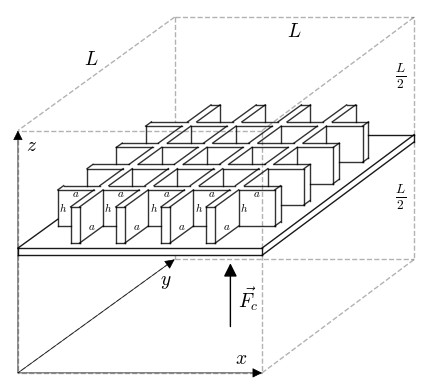
\includegraphics[width=0.48\textwidth]{honeycomb_box_L.png}
%\caption{}{Cubic cavity with a plate \\ covered by honeycomb}
%\end{center}
%\label{fig:honeycomb_box_L}
% \end{wrapfigure}

\vspace{\myvspacebeforesubsection}
    \subsection*{\centering{\fontencoding{T1}\fontfamily{ptm}{\selectfont \uppercase{Two dimensional Casimir's
approach}}}} \label{two-dimensional-casimirs-approach}
\vspace{\myvspaceaftersubsection}

% \begin{multicols}{2}

    Let us consider a cubic cavity of volume \(L^3\) bounded by perfectly
conducting walls where perfectly conducting square plate with side
\(L\) is placed in this cavity parallel to the \(xy\) face, and let
the distance between the plate and the \(xy\) face be sufficiently large,
\(L/2\), for example.
One side of this perfectly conducting square plate is a smooth plane and
another is covered with perfectly conducting square-shaped honeycombs with
a square side \(a\).

On both sides of the plate the expressions \(\sum\hbar\omega\big/2\)
where the summation extends over all possible resonance frequencies of
the cavity \(L/2 \times L \times L\) (a large cavity: between smooth plane
and \(xy\) face) and the cavity \(L/2 \times a\times a\) (a small
cavity, one honeycomb cell: between the bottom of the honeycomb and the
opposite \(xy\) face) are divergent and devoid of physical meaning but
the difference between these sums on the opposite sides of the plate,
\(\left(\sum\,\,\hbar\omega\right)_{I}\big/{\left(2\,V_{I}\right)} - \left(\sum\,\,\hbar\omega\right)_{II}\big/{\left(2\,V_{II}\right)}\),
will be shown to have a well-defined value and this value will be
interpreted as the interaction between the plate and the both remote
\(xy\) faces.

    The possible oscillations inside cavities defined by
\(0 \leq x \leq L\), \(0 \leq y \leq L\), \(0 \leq z \leq L/2\) (a large cavity between smooth
plane and \(xy\) face) and
\(0 \leq x \leq a\), \(0 \leq y \leq a\), \(0 \leq z \leq L/2\) (a small cavity, one honeycomb
cell) have wave vectors
\(k_x = \frac{\pi}{L}\,n_x\), \(k_y = \frac{\pi}{L}\,n_y\),
\(k_z = \frac{\pi}{L/2}\,n_z\) (a large cavity between smooth plane and
\(xy\) face), and
\(k_x = \frac{\pi}{a}\,n_x\), \(k_y = \frac{\pi}{a}\,n_y\),
\(k_z = \frac{\pi}{L/2}\,n_z\) (a small cavity, one honeycomb cell),
where \(n_x\), \(n_y\), \(n_z\) are positive integers;
    \(k = \sqrt{k_x^2+k_y^2+k_z^2} = \sqrt{\kappa^2+k_z^2}\).

\begin{figure}
\begin{center}
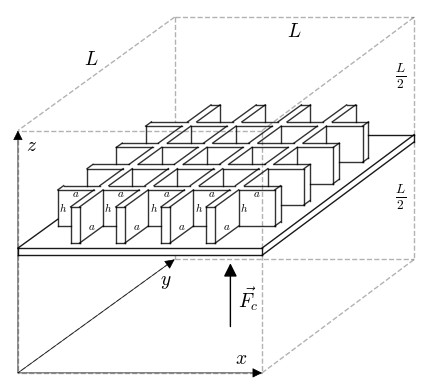
\includegraphics[width=0.42\textwidth]{honeycomb_box_L.png}
\caption{}{\centering{\textbf{Fig.1.} Cubic cavity with a plate covered by honeycomb.}}
\end{center}
\label{fig:honeycomb_box_L}
\end{figure}


Let us write the expression for the sum of zero-point energy in general form

\vspace{-3.5mm}
\begin{equation} \label{eq:1}
E = \frac{1}{2}\sum\,\hbar\omega = \hbar\,c\frac{1}{2}\sum\limits_{n_x}^{}\sum\limits_{n_y}^{}\sum\limits_{n_z}^{}k.
\end{equation}
\vspace{-3.5mm}

    Two standing waves correspond to every \(k_x\), \(k_y\), \(k_z\) but in case when one of the \(n_i\) is zero, there is only one wave.

    That is of no importance in case of one honeycomb cell cavity for \(k_z\),
since for very large \(L/2\) we may regard \(k_z\) as
continuous variable, replacing summation over \(n_z\) with integration.
Thus, for a small cavity consisting of one honeycomb, we find

\noindent
\(E = \frac{\hbar\,c}{2}\int\limits_{0}^{\infty}\left[{\sqrt{k_z^2}+2\sum\limits_{n_x=1}^{\infty}\sum\limits_{n_y=1}^{\infty}\sqrt{\frac{n_x^2 \pi^2}{a^2}+\frac{n_y^2 \pi^2}{a^2}+k_z^2}}\right]d{n_z}\).

   Considering \(dn_z = \frac{L/2}{\pi}\,dk_z\) we can find the specific energy density \(E/V\), where
\(V = V_{small} = a^2 L/2\):

    % \(\frac{1}{2\,V}\sum\,\hbar\omega = \frac{\hbar\,c}{a^2\,L/2}\frac{1}{2}\int\limits_{0}^{\infty}\left[{\sqrt{k_z^2}+2\sum\limits_{n_x=1}^{\infty}\sum\limits_{n_y=1}^{\infty}\sqrt{n_x^2\frac{\pi^2}{a^2}+n_y^2\frac{\pi^2}{a^2}+k_z^2}}\right]\frac{L/2}{\pi}\,dk_z\)
% (small cavity, one honeycomb cell),

\noindent
\(\frac{E}{V} = \frac{\hbar\,c}{a^2\,\pi}\int\limits_{0}^{\infty}\left[{\frac{\sqrt{k_z^2}}{2}+\sum\limits_{n_x=1}^{\infty}\sum\limits_{n_y=1}^{\infty}\sqrt{\frac{n_x^2 \pi^2}{a^2}+\frac{n_y^2 \pi^2}{a^2}+k_z^2}}\right] dk_z\),
%(small cavity, one honeycomb cell),

\noindent
\(\frac{E}{V} = \frac{\hbar\,c}{a^2\,\pi}\int\limits_{0}^{\infty}\left[{\sum\limits_{n_x=(0)1}^{\infty}\sum\limits_{n_y=(0)1}^{\infty}\sqrt{n_x^2\frac{\pi^2}{a^2}+n_y^2\frac{\pi^2}{a^2}+k_z^2}}\right] dk_z\),
%(small cavity, one honeycomb cell),

    where the notation \(\left(0\right) 1\) is meant to indicate that the
term with \(n_x = 0\) and \(n_y = 0\) has to be multiplied by
\(1\big/2\). Thus, for a small cavity consisting of one honeycomb, we have

    \(\frac{E}{V} = \frac{\hbar\,c}{a^2\,\pi}\sum\limits_{n_x=(0)1}^{\infty}\sum\limits_{n_y=(0)1}^{\infty}\left[\int\limits_{0}^{\infty}\sqrt{n_x^2\frac{\pi^2}{a^2}+n_y^2\frac{\pi^2}{a^2}+k_z^2}\,dk_z\right]\).
%(small cavity, one honeycomb cell),

    That is of no importance in case of a large cavity for \(k_x\), \(k_y\)
since for very large \(L\) we may regard \(k_x\), \(k_y\) as
continuous variables. Thus, for large cavity between smooth plane and \(xy\) face we find
\noindent
\(\begin{array}{c}
\begin{array}{ll}
    \sum\frac{\hbar\omega}{2} = & \frac{\hbar c}{2}\int\limits_{0}^{\infty}\int\limits_{0}^{\infty}\Bigg[\sqrt{k_x^2+k_y^2}\,+ \\
   & +\,2\sum\limits_{n_z=1}^{\infty}\sqrt{\frac{n_z^2 \pi^2}{(L/2)^2}+k_x^2+k_y^2}\Bigg]d{n_x}d{n_y}.
\end{array}
\end{array}\)

%(large cavity between pure plane and \(xy\) face),

    For very large \(L/2\) the last summation may also be replaced by an
integral and, therefore, it can be seen that energy of a large cavity is given by

    \(\frac{1}{2}\sum\,\hbar\omega = \hbar\,c\int\limits_{0}^{\infty}\int\limits_{0}^{\infty}\int\limits_{0}^{\infty}\sqrt{k_z^2+k_x^2+k_y^2}\,d{n_x}\,d{n_y}\,d{n_z}\),
%(large cavity between pure plane and \(xy\) face),

    \(dn_x = \frac{L}{\pi}\,dk_x\), \(dn_y = \frac{L}{\pi}\,dk_y\),
\(dn_z = \frac{L/2}{\pi}\,dk_z\),

    Now for the specific energy density \(E/V\) for a large cavity, where
\(V = V_{large} = L^3/2\) we can write the following sequence of transformations:

\noindent
    \(\frac{E}{V} = \frac{\hbar\,c}{L^3/2}\int\limits_{0}^{\infty}\int\limits_{0}^{\infty}\int\limits_{0}^{\infty}\sqrt{k_z^2+k_x^2+k_y^2}\,dn_x\,dn_y\,\frac{L/2}{\pi}\,dk_z\),
%(large cavity between pure plane and \(xy\) face),

    % \(\frac{1}{2\,V}\sum\,\hbar\omega = \frac{\hbar\,c}{L^2\,\pi}\int\limits_{0}^{\infty}\int\limits_{0}^{\infty}\left[\,\int\limits_{0}^{\infty}\sqrt{k_z^2+k_x^2+k_y^2}\,dk_z\right]\,dn_x\,dn_y\)
% (large cavity between pure plane and \(xy\) face),
%\noindent
%    \(\frac{E}{V} = \frac{\hbar\,c}{L^2\,\pi}\int\limits_{0}^{\infty}\int\limits_{0}^{\infty}\left[\,\int\limits_{0}^{\infty}\sqrt{k_x^2+k_y^2+k_z^2}\,dk_z\right]\,dn_x\,dn_y\),
%(large cavity between pure plane and \(xy\) face),

\noindent
    \(\frac{E}{V} = \frac{\hbar\,c}{L^2\,\pi}\int\limits_{0}^{\infty}\int\limits_{0}^{\infty}\left[\,\int\limits_{0}^{\infty}\sqrt{k_x^2+k_y^2+k_z^2}\,dk_z\right]\,\left(\frac{L}{\pi}dk_x\right)\,\left(\frac{L}{\pi}dk_y\right)\),
%(large cavity between pure plane and \(xy\) face),

\noindent
    \(\frac{E}{V} = \frac{\hbar\,c}{a^2\,\pi}\int\limits_{0}^{\infty}\int\limits_{0}^{\infty}\left[\,\int\limits_{0}^{\infty}\sqrt{k_x^2+k_y^2+k_z^2}\,dk_z\right]\,\left(\frac{a}{\pi}dk_x\right)\,\left(\frac{a}{\pi}dk_y\right)\).
%(large cavity between pure plane and \(xy\) face),

And finally for a large cavity between smooth plane and \(xy\) face we can formulate the energy density as following

    \(\frac{\sum\,\hbar\omega}{2\,V} = \frac{\hbar\,c}{a^2\,\pi}\int\limits_{0}^{\infty}\int\limits_{0}^{\infty}\left[\,\int\limits_{0}^{\infty}\sqrt{k_x^2+k_y^2+k_z^2}\,dk_z\right]\,dn_x\,dn_y\),

but for a small cavity, one honeycomb cell we have
\noindent
    \(\frac{\sum\,\hbar\omega}{2\,V} = \frac{\hbar\,c}{a^2\,\pi}\sum\limits_{n_x=(0)1}^{\infty}\sum\limits_{n_y=(0)1}^{\infty}\left[\,\int\limits_{0}^{\infty}\sqrt{n_x^2\frac{\pi^2}{a^2}+n_y^2\frac{\pi^2}{a^2}+k_z^2}\,dk_z\right]\).


%    \({\left(\frac{E}{V}\right)_{small\,cavity} = \frac{\hbar}{a^2} \sum\limits_{n_x=(0)1}^{\infty}\sum\limits_{n_y=(0)1}^{\infty}\,\int\limits_{0}^{\infty} {\frac {dk_{z}}{\pi}}\,\omega _{n_x,n_y},}\)

%    where
%\(\omega _{n_x,n_y} = c\,\sqrt{n_x^2\frac{\pi^2}{a^2}+n_y^2\frac{\pi^2}{a^2}+k_z^2}\)

Therefore, it is obvious that the interaction energy is determined by the following energy density difference:
%    \[\begin{array}{lr}
%\delta\,\frac{E}{V} =
%\begin{array}{c}
%\frac{\hbar\,c}{a^2\,\pi}\Bigg\{\sum\limits_{n_x=(0)1}^{\infty}\sum\limits_{n_y=(0)1}^{\infty}\left[\,\int\limits_{0}^{\infty}\sqrt{n_x^2\frac{\pi^2}{a^2}+n_y^2\frac{\pi^2}{a^2}+k_z^2}\,dk_z\right] - \\
%\int\limits_{0}^{\infty}\int\limits_{0}^{\infty}\left[\,\int\limits_{0}^{\infty}\sqrt{k_x^2+k_y^2+k_z^2}\,dk_z\right]\,\left(\frac{a}{\pi}dk_x\right)\,\left(\frac{a}{\pi}dk_y\right)\Bigg\}
%\end{array}\end{array}\]
\end{multicols}
\noindent

\vspace{-3.5mm}
    \begin{equation} \label{eq:2}
\begin{array}{lr}
\delta \frac{E}{V} =
\begin{array}{c}
\frac{\hbar c}{a^2 \pi}\Bigg\{\sum\limits_{n_x=(0)1}^{\infty}\sum\limits_{n_y=(0)1}^{\infty}\left[\int\limits_{0}^{\infty}\sqrt{\frac{n_x^2 \pi^2}{a^2}+\frac{n_y^2 \pi^2}{a^2}+k_z^2} dk_z\right] % \\ 
-\int\limits_{0}^{\infty}\int\limits_{0}^{\infty}\left[\int\limits_{0}^{\infty}\sqrt{k_x^2+k_y^2+k_z^2}\,dk_z\right] dn_x dn_y\Bigg\}.
\end{array}\end{array}\end{equation}
\vspace{-3.5mm}

\begin{multicols}{2}

    This expression is clearly infinite, and to proceed with the
calculation, it is convenient to introduce a regulator.

    In order to receive a finite result, it is necessary to multiply the
integrands by a regularization function \(f(k/k_m)\) which is unity for
\(k << k_m\) but tends to zero sufficiently rapidly for
\((k/k_m)\, \rightarrow\,\infty\). Where \(k_m\) may be defined by
\(f(1) = {1}/{2}\). The physical meaning is obvious: our plate is hardly an obstacle for very short
waves (X-rays e.g.) and, therefore, the zero-point energy of these waves will not be
influenced by the position of this plate.

    The purpose of regulator is to make the expression finite, and
influence of its specific type will be removed by a limit transition in the end.

    Introducing the variable \(u^2 = a^2\,k_z^2/\pi^2\),
\(du = a/\pi\,dk_z\), we have:
\end{multicols}
\vspace{-3.5mm}
    \begin{equation} \label{eq:3}
\begin{array}{c}
\begin{array}{ll}
\delta\,\frac{E}{V} =
\frac{\hbar\,c\,\pi}{a^4}\Bigg\{
\sum\limits_{n_x=\left(0\right)\,1}^{\infty}
\sum\limits_{n_y=\left(0\right)\,1}^{\infty}
\int\limits_{0}^{\infty}
{\sqrt{n_x^2 + n_y^2 + u^2}} &
f\left(\frac{\pi\sqrt{n_x^2 + n_y^2 + u^2}}{a\,k_m}\right)
\,d{u} \\
\, &- \int\limits_{0}^{\infty}
\int\limits_{0}^{\infty}
\int\limits_{0}^{\infty}
{\sqrt{n_x^2 + n_y^2 + u^2}}
f\left(\frac{\pi\sqrt{n_x^2 + n_y^2 + u^2}}{a\,k_m}\right)
\,d{u}\,d{n_x}\,d{n_y}
\Bigg\}.
\end{array}
\end{array}
\end{equation}
\vspace{-3.5mm}
\begin{multicols}{2}
    If \(\omega _{n_x,n_y} = c\,\sqrt{n_x^2\frac{\pi^2}{a^2}+n_y^2\frac{\pi^2}{a^2}+k_z^2}\)
and \(k_z^2 = u^2 \frac{\pi^2}{a^2}\) we have
\(\omega _{n_x,n_y} = c \, \frac{\pi}{a} \sqrt{n_x^2+n_y^2+u^2}\) so
\(f\left(\frac{\pi\sqrt{n_x^2 + n_y^2+u^2}}{a\,k_m}\right) = f\left(\frac{\omega _{n_x,n_y}}{c\,k_m}\right)\),
where the cutting frequency is \(\omega_m = c\,k_m\).
    Introducing function
\noindent
\begin{equation} \label{eq:4}
F = %\left(u, n_x, n_y\right) =
\sqrt{n_x^2 + n_y^2+u^2}\,
f\left(\frac{\pi\sqrt{n_x^2 + n_y^2+u^2}}{a\,k_m}\right)
\end{equation}

    we can write

\noindent
$\begin{array}{c}
\begin{array}{ll}
\delta\,\frac{E}{V} =
\frac{\hbar\,c\,\pi}{a^4}
&\Bigg\{
\sum\limits_{n_x=\left(0\right)\,1}^{\infty}
\sum\limits_{n_y=\left(0\right)\,1}^{\infty}
\left(\int\limits_{0}^{\infty}F\left(u, n_x, n_y\right)\,d{u}\right)
\\
\, & \,\,\,\,\,\, - \int\limits_{0}^{\infty}
\int\limits_{0}^{\infty}
\left(\int\limits_{0}^{\infty}F\left(u, n_x, n_y\right)\,d{u}\right)
\,d{n_x}\,d{n_y}
\Bigg\}.
\end{array}
\end{array}$

    And at least, introducing
\noindent
\begin{equation} \label{eq:5}
G\left(n_x, n_y\right) = \int\limits_{0}^{\infty}F\left(u, n_x, n_y\right)\,d{u}
\end{equation}

    we have

    \begin{equation} \label{eq:6}
\begin{array}{lr}
\delta\,\frac{E}{V} =
\begin{array}{c}
 \frac{\hbar\,c\,\pi}{a^4} \Bigg\{
\sum\limits_{n_x=\left(0\right)\,1}^{\infty}
\sum\limits_{n_y=\left(0\right)\,1}^{\infty}
G\left(n_x, n_y\right)
\\
- \int\limits_{0}^{\infty}
\int\limits_{0}^{\infty}
G\left(n_x, n_y\right)
\,d{n_x}\,d{n_y}
\Bigg\}.
\end{array}
\end{array}
\end{equation}

Integration of \(G\left(n_x, n_y\right)\) with example of regulator
function is presented in Appendix A.

    To receive a way of calculating \(\delta\left(E/V\right)\), the Euler-Maclaurin 2D formula
could be considered.

% \end{multicols}

\vspace{\myvspacebeforesubsection}
\subsection*{\centering{\fontencoding{T1}\fontfamily{ptm}{\selectfont \uppercase{Euler-Maclaurin 2D formula}}}} \label{eulermaclaurin-2d-formula}
\vspace{\myvspaceaftersubsection}

% \begin{multicols}{2}

According to A.Bikyalis \cite{Bikyalis1968} we apply Euler-Maclaurin
formula twice on \(n_x\) and on \(n_y\). Starting from the following form of this formula

% \[{\displaystyle \sum _{i=a}^{b}f(i)=\int\limits_{a}^{b}f(x)\,dx+{\frac {f(a)+f(b)}{2}}+\sum\limits_{k=1}^{\lfloor p/2\rfloor }{\frac {B_{2k}}{(2k)!}}\left(f^{(2k-1)}(b)-f^{(2k-1)}(a)\right)+R_{p},}\]

    \begin{equation} \label{eq:7}
\begin{array}{l}
\begin{array}{ll}
\displaystyle \sum _{i=a}^{b}f(i)= \int_{a}^{b}f(x)\,dx+{\frac {f(a)+f(b)}{2}} + & \,\,\,\,
\end{array}  \\
\begin{array}{rr}
\,\,\, & +\,\sum_{k=1}^{\lfloor p/2\rfloor }{\frac {B_{2k}}{(2k)!}}\left(f^{(2k-1)}(b)-f^{(2k-1)}(a)\right)+ \\
\,\,\, & + \,R_{p},
\end{array}
\end{array}\end{equation}

\begin{equation} \label{eq:8}
{\displaystyle P_{k}(x)=B_{k}\left(x-\lfloor x\rfloor \right),}
\end{equation}

\begin{equation} \label{eq:9}
{\displaystyle R_{p}=(-1)^{p+1}\int_{a}^{b}f^{(p)}(x){\frac {P_{p}(x)}{p!}}\,dx},
\end{equation}

since we are dealing with a very complex mathematical
problem of integrating the function, which often oscillates and
suffers discontinuities at the points of each integer value of the
argument due to the presence of the multiplier \((x-\lfloor x\rfloor )\), hereafter,
we will use the fact that the remainder can also
be expressed in the form

\begin{equation} \label{eq:10}
{\displaystyle R_{p}=(-1)^{p+1}\sum_{j=a}^{b-1} \int _{0}^{1}f^{(p)}(v+j){\frac {B_{p}(v)}{p!}}\,dv}.
\end{equation}

We can see that it consists of 4 parts:

\noindent
the integral \(\int\limits_{x}^{}=\int _{x_a}^{x_b}f(x)\,dx\),

\noindent
the half sum \(\underset{x}{H_{\sum}}={\left( {f(x_a)+f(x_b)}\right)/{2}}\),

\noindent
the sum of Bernoulli polynomials

\({\sum\limits_{x}^{}}^{B}=\sum _{k=1}^{\lfloor p/2\rfloor }{\frac {B_{2k}}{(2k)!}}\left(f^{(2k-1)}(x_b)-f^{(2k-1)}(x_a)\right)\),

\noindent
and the remainder

\(\underset{x}{R_{p}}=(-1)^{p+1}\sum_{j=x_a}^{x_b-1} \int _{0}^{1}f^{(p)}(v_x+j_x){\frac {B_{p}(v_x)}{p!}}\,dv_x\).

When applying it to \(G\) twice on \(n_x\) and on \(n_y\) we should have
the following summands which can be represented as the table:

    \begin{equation} \label{eq:11}
\begin{array}{cccc}
 \int\limits_{n_y}^{} \int\limits_{n_x}^{} G  &  \int\limits_{n_y}^{} \underset{n_x}{H_{\sum}}\,G  &  \int\limits_{n_y}^{}{\sum\limits_{n_x}^{}}^{B}\,G  &  \int\limits_{n_y}^{}\,\underset{n_x}{R_{p}}\,G  \\
 \underset{n_y}{H_{\sum}}\,\int\limits_{n_x}^{}\,G &  \underset{n_y}{H_{\sum}}\,\underset{n_x}{H_{\sum}}\,G &  \underset{n_y}{H_{\sum}}\,{\sum\limits_{n_x}^{}}^{B}\,G &  \underset{n_y}{H_{\sum}}\,\underset{n_x}{R_{p}}\,G \\
 {\sum\limits_{n_y}^{}}^{B}\,\int\limits_{n_x}^{}\,G  &  {\sum\limits_{n_y}^{}}^{B}\,\underset{n_x}{H_{\sum}}\,G  &  {\sum\limits_{n_y}^{}}^{B}\,{\sum\limits_{n_x}^{}}^{B}\,G  &  {\sum\limits_{n_y}^{}}^{B}\,\underset{n_x}{R_{p}}\,G  \\
 \underset{n_y}{R_{p}}\,\int\limits_{n_x}^{}\,G   &  \underset{n_y}{R_{p}}\,\underset{n_x}{H_{\sum}}\,G   &  \underset{n_y}{R_{p}}\,{\sum\limits_{n_x}^{}}^{B}\,G   &  \underset{n_y}{R_{p}}\,\underset{n_x}{R_{p}}\,G.
\end{array}\end{equation}

    Taking into account that the function \(G\) is symmetric on
its \(n_x\) and \(n_y\) arguments, so the two-dimentional
Euler-Maclaurin marix presented above is symmetric too.

% \end{multicols}

\vspace{\myvspacebeforesubsection}
    \subsection*{\centering{\fontencoding{T1}\fontfamily{ptm}{\selectfont \uppercase{Summary of Euler-Maclaurin
2D}}}} \label{summary-of-eulermaclaurin-2d}
\vspace{\myvspaceaftersubsection}

% \begin{multicols}{2}

Taking value of parameter \(p = 1\) we have:

    \begin{center}
\begin{tabular}{ l }
%\hline

$\int\limits_{n_y}^{} \int\limits_{n_x}^{} G = \int\limits_{a_{y}}^{b_{y}} \int\limits_{a_{x}}^{b_{x}} G\left(n_{x}, n_{y}\right)\,{d n_{x}}\,{d n_{y}}$ \\

$\int\limits_{n_y}^{} \underset{n_x}{H_{\sum}}\,G = \frac{1}{2} \, \int\limits_{a_{y}}^{b_{y}} G\left(a_{x}, n_{y}\right)\,{d n_{y}}$ \\

$\int\limits_{n_y}^{} {\sum\limits_{n_x}^{}}^{B}\,G = 0$ \\

$\int\limits_{n_y}^{} \underset{n_x}{R_{p}}\,G = {\sum\limits_{j_{x}=a_{x}}^{b_{x} - 1} \int\limits_{a_{y}}^{b_{y}} \int\limits_{0}^{1} \frac{1}{2} \, {\left(2 \, v_{n_{x}} - 1\right)} G'\left(\widehat{j_{x} + v_{n_{x}}}, n_{y}\right){d v_{n_{x}}}{d n_{y}}}$ \\

%\hline

\end{tabular}
\end{center}

    \begin{center}
\begin{tabular}{ l }

%\hline

$\underset{n_y}{H_{\sum}}\,\int\limits_{n_x}^{}\,G = \frac{1}{2} \, \int\limits_{a_{x}}^{b_{x}} G\left(n_{x}, a_{y}\right)\,{d n_{x}}$ \\

$\underset{n_y}{H_{\sum}}\,\underset{n_x}{H_{\sum}}\,G = \frac{1}{4} \, G\left(a_{x}, a_{y}\right)$ \\

$\underset{n_y}{H_{\sum}}\,{\sum\limits_{n_x}^{}}^{B}\,G = 0$ \\

$\underset{n_y}{H_{\sum}}\,\underset{n_x}{R_{p}}\,G = {\sum\limits_{j_{n_{x}}=a_{x}}^{b_{x} - 1} \frac{1}{4} \, \int\limits_{0}^{1} \left(2 \, v_{n_{x}} - 1 \right) G'\left(\widehat{j_{n_{x}} + v_{n_{x}}}, a_{y}\right)\,{d v_{n_{x}}} }$ \\

%\hline

\end{tabular}
\end{center}

    \begin{center}
\begin{tabular}{ l }

%\hline

${\sum\limits_{n_y}^{}}^{B}\,\int\limits_{n_x}^{}\,G = 0$ \\

${\sum\limits_{n_y}^{}}^{B}\,\underset{n_x}{H_{\sum}}\,G = 0$ \\

${\sum\limits_{n_y}^{}}^{B}\,{\sum\limits_{n_x}^{}}^{B}\,G = 0$ \\

${\sum\limits_{n_y}^{}}^{B}\,\underset{n_x}{R_{p}}\,G = 0$ \\

%\hline

\end{tabular}
\end{center}

    \begin{center}
\begin{tabular}{ l }

%\hline

$\underset{n_y}{R_{p}}\,\int\limits_{n_x}^{}\,G = {\sum\limits_{j_{x}=a_{x}}^{b_{x} - 1} \int\limits_{a_{y}}^{b_{y}} \int\limits_{0}^{1} \frac{1}{2} \, {\left(2 \, v_{n_{x}} - 1\right)} G'\left(\widehat{j_{x} + v_{n_{x}}}, n_{y}\right){d v_{n_{x}}}{d n_{y}}}$ \\

$\underset{n_y}{R_{p}}\,\underset{n_x}{H_{\sum}}\,G = {\sum\limits_{j_{n_{y}}=a_{y}}^{b_{y} - 1} \int\limits_{0}^{1} \frac{1}{4} \, {\left(2 \, v_{n_{y}} - 1\right)} G'\left(a_{x}, \widehat{j_{n_{y}} + v_{n_{y}}}\right)\,{d v_{n_{y}}}}$ \\

$\underset{n_y}{R_{p}}\,{\sum\limits_{n_x}^{}}^{B}\,G = 0$ \\

%$\underset{n_y}{R_{p}}\,\underset{n_x}{R_{p}}\,G = {\sum\limits_{j_{y}=a_{y}}^{b_{y} - 1} {\sum\limits_{j_{x}=a_{x}}^{b_{x} - 1} \int\limits_{0}^{1} \int\limits_{0}^{1}\frac{1}{4} {\left(2 \, v_{y} - 1\right)} {\left(2 \, v_{x} - 1\right)} 
%G''\left(\widehat{j_{x} + v_{x}}, \widehat{j_{y} + v_{y}}\right)\,{d v_{x}}}\,{d v_{y}}}$ \\


$\begin{array}{lr}
\underset{n_y}{R_{p}}\,\underset{n_x}{R_{p}}\,G =
\begin{array}{c}
 \sum\limits_{j_{y}=a_{y}}^{b_{y} - 1} \sum\limits_{j_{x}=a_{x}}^{b_{x} - 1} \int\limits_{0}^{1} \int\limits_{0}^{1}\frac{1}{4} \left(2 \, v_{y} - 1\right)  \left(2 \, v_{x} - 1\right) \cdot \\
G''\left(\widehat{j_{x} + v_{x}}, \widehat{j_{y} + v_{y}}\right)\,{d v_{x}}\,{d v_{y}}
\end{array}
\end{array}$ \\


%\hline

\end{tabular}
\end{center}

% \end{multicols}

\vspace{\myvspacebeforesubsection}
    \subsection*{\centering {\fontencoding{T1}\fontfamily{ptm}{\selectfont {\uppercase{A way \\ of calculating~}\(\delta\left(E/V\right)\)}}}}\label{a-way-of-calculating-deltaleftevright}
\vspace{\myvspaceaftersubsection}

% \begin{multicols}{2}

    Let us consider the expression

\begin{equation} \label{eq:12}
\sum\limits_{n_x=\left(0\right)\,1}^{\infty}
\sum\limits_{n_y=\left(0\right)\,1}^{\infty}
G%\left(n_x, n_y\right)
-
\int\limits_{0}^{\infty}
\int\limits_{0}^{\infty}
G%\left(n_x, n_y\right)
\,\,\,d{n_x}\,d{n_y}
\end{equation}

    Firstly, we can see, that

\begin{equation} \label{eq:13}
\begin{array}{c}
    \sum\limits_{n_x=\left(0\right)\,1}^{\infty} \sum\limits_{n_y=\left(0\right)\,1}^{\infty} {G\left(n_x, n_y\right)} = \\
% \sum\limits_{n_x=\left(0\right)\,1}^{\infty} \left( -\frac{1}{2}G\left(n_x, 0\right) + \sum\limits_{n_y=0}^{\infty}{G\left(n_x, n_y\right)} \right) = \\
% -\frac{1}{2} \left( -\frac{1}{2}G\left(0, 0\right) + \sum\limits_{n_y=0}^{\infty}{G\left(0, n_y\right)} \right) + \\
%\sum\limits_{n_x=0}^{\infty} \left( -\frac{1}{2}G\left(n_x, 0\right) + \sum\limits_{n_y=0}^{\infty}{G\left(n_x, n_y\right)} \right) = \\
 \frac{1}{4}G\left(0, 0\right) - \frac{1}{2}\sum\limits_{n_y=0}^{\infty}{G\left(0, n_y\right)}\, - \\
\frac{1}{2}\sum\limits_{n_x=0}^{\infty}{G\left(n_x, 0\right)} + \sum\limits_{n_x=0}^{\infty}\sum\limits_{n_y=0}^{\infty}{G\left(n_x, n_y\right)}.
\end{array}
\end{equation}

    Therefore, we have

\noindent
\(\begin{array}{l}
\begin{array}{ll}
\sum\limits_{n_x=\left(0\right)\,1}^{\infty} \sum\limits_{n_y=\left(0\right)\,1}^{\infty} G\left(n_x, n_y\right)
 - \\
\,\,\,\,\,\,\,\,\,\,\,\,\,\,\,\,\,\,\,\,\,\,\,\,\,\,\,\,\,\,\,\,\,\,\,\,\,\,\,\,\,\,\,\,\,\,\,\,\,\,\,\int\limits_{0}^{\infty} \int\limits_{0}^{\infty} G\left(n_x, n_y\right)\,d{n_x}\,d{n_y} = & \, \\
\end{array} \\
\begin{array}{c}
\frac{1}{4}G\left(0, 0\right) -\frac{1}{2}\sum\limits_{n_y=0}^{\infty}{G\left(0, n_y\right)} -\frac{1}{2}\sum\limits_{n_x=0}^{\infty}{G\left(n_x, 0\right)}\, + \\
\end{array} \\
\begin{array}{rr}
\, & \sum\limits_{n_x=0}^{\infty}\sum\limits_{n_y=0}^{\infty}{G\left(n_x, n_y\right)} - \int\limits_{0}^{\infty} \int\limits_{0}^{\infty} G\left(n_x, n_y\right)\,d{n_x}\,d{n_y}.
\end{array}
\end{array}\)

    On the other hand, we have found that

\noindent
\(\sum\limits_{n_x=0}^{\infty} \sum\limits_{n_y=0}^{\infty} G\left(n_x, n_y\right) -\int\limits_{0}^{\infty} \int\limits_{0}^{\infty} G\left(n_x, n_y\right)\,d{n_x}\,d{n_y} = \\
 \begin{array}{cccc}  \, &  \int\limits_{n_y}^{} \underset{n_x}{H_{\sum}}\,G &  + \int\limits_{n_y}^{}{\sum\limits_{n_x}^{}}^{B}\,G &  + \int\limits_{n_y}^{}\,\underset{n_x}{R_{p}}\,G \\
  +\underset{n_y}{H_{\sum}}\,\int\limits_{n_x}^{}\,G &  + \underset{n_y}{H_{\sum}}\,\underset{n_x}{H_{\sum}}\,G &  + \underset{n_y}{H_{\sum}}\,{\sum\limits_{n_x}^{}}^{B}\,G &  + \underset{n_y}{H_{\sum}}\,\underset{n_x}{R_{p}}\,G \\
  + {\sum\limits_{n_y}^{}}^{B}\,\int\limits_{n_x}^{}\,G &  + {\sum\limits_{n_y}^{}}^{B}\,\underset{n_x}{H_{\sum}}\,G &  + {\sum\limits_{n_y}^{}}^{B}\,{\sum\limits_{n_x}^{}}^{B}\,G &  + {\sum\limits_{n_y}^{}}^{B}\,\underset{n_x}{R_{p}}\,G \\
  + \underset{n_y}{R_{p}}\,\int\limits_{n_x}^{}\,G &  + \underset{n_y}{R_{p}}\,\underset{n_x}{H_{\sum}}\,G &  + \underset{n_y}{R_{p}}\,{\sum\limits_{n_x}^{}}^{B}\,G &  + \underset{n_y}{R_{p}}\,\underset{n_x}{R_{p}}\,G, \end{array}\)

    where \(\underset{n_y}{H_{\sum}}\,\underset{n_x}{H_{\sum}}\,G\),
\(\int\limits_{n_y}^{} \underset{n_x}{H_{\sum}}\,G\) and
\(\underset{n_y}{H_{\sum}}\,\int\limits_{n_x}^{}\,G\) are:

\noindent
    \(\frac{1}{4} \, G\left(a_{x}, a_{y}\right) , \frac{1}{2} \, \int_{a_{y}}^{b_{y}} G\left(a_{x}, n_{y}\right)\,{d n_{y}} , \frac{1}{2} \, \int_{a_{x}}^{b_{x}} G\left(n_{x}, a_{y}\right)\,{d n_{x}}.\)

    Now using 1D Euler-Maclaurin formula in the form (\ref{eq:7}) we can see that

%\noindent
%$\begin{array}{l}
%\begin{array}{ll}
%\displaystyle \sum _{i=a}^{b}f(i)=\int _{a}^{b}f(x)\,dx+{\frac {f(a)+f(b)}{2}}+ & \, \\
%\end{array} \\
%\begin{array}{rr}
%\, &
%\sum _{k=1}^{\lfloor p/2\rfloor }{\frac {B_{2k}}{(2k)!}}(f^{(2k-1)}(b)-f^{(2k-1)}(a))+R_{p},
%\end{array}
%\end{array}$

    

    \[
\frac{1}{4}G\left(0, 0\right)
- \frac{1}{2}\sum\limits_{n_y=0}^{\infty}{G\left(0, n_y\right)}
- \frac{1}{2}\sum\limits_{n_x=0}^{\infty}{G\left(n_x, 0\right)}
\]

    will be equal to

\noindent
\(\begin{array}{l}
    \begin{array}{l}
  \underset{n_y}{H_{\sum}} \underset{n_x}{H_{\sum}} G \\
\end{array} \\
\begin{array}{rrrrr}
  \, &  - \int\limits_{n_y}^{} \underset{n_x}{H_{\sum}}\,G &  - \underset{n_y}{H_{\sum}} \underset{n_x}{H_{\sum}}\,G &  - \frac{1}{2}{\sum\limits_{n_y}^{}}^{B}\,G &  - \frac{1}{2}\underset{n_y}{R_{p}}\,G/2 \\
  \,&  - \underset{n_y}{H_{\sum}}\int\limits_{n_x}^{} \,G &  - \underset{n_y}{H_{\sum}} \underset{n_x}{H_{\sum}}\,G &  - \frac{1}{2}{\sum\limits_{n_x}^{}}^{B}\,G &  - \frac{1}{2}\underset{n_x}{R_{p}}\,G/2. \\
\end{array}
\end{array}\)

    Now we can find expression (\ref{eq:12}) by using the following summation

%\(\sum\limits_{n_x=\left(0\right)\,1}^{\infty} \sum\limits_{n_y=\left(0\right)\,1}^{\infty} G\left(n_x, n_y\right) - \int\limits_{0}^{\infty} \int\limits_{0}^{\infty} G\left(n_x, n_y\right)\,d{n_x}\,d{n_y}\)



\noindent
    \(\begin{array}{llll}  \,&  \,&  + \int\limits_{n_y}^{}{\sum\limits_{n_x}^{}}^{B}\,G &  + \int\limits_{n_y}^{}\,\underset{n_x}{R_{p}}\,G \\  \,&  \,&  + \underset{n_y}{H_{\sum}}\,{\sum\limits_{n_x}^{}}^{B}\,G &  + \underset{n_y}{H_{\sum}}\,\underset{n_x}{R_{p}}\,G \\  + {\sum\limits_{n_y}^{}}^{B}\,\int\limits_{n_x}^{}\,G &  + {\sum\limits_{n_y}^{}}^{B}\,\underset{n_x}{H_{\sum}}\,G &  + {\sum\limits_{n_y}^{}}^{B}\,{\sum\limits_{n_x}^{}}^{B}\,G &  + {\sum\limits_{n_y}^{}}^{B}\,\underset{n_x}{R_{p}}\,G \\  + \underset{n_y}{R_{p}}\,\int\limits_{n_x}^{}\,G &  + \underset{n_y}{R_{p}}\,\underset{n_x}{H_{\sum}}\,G &  + \underset{n_y}{R_{p}}\,{\sum\limits_{n_x}^{}}^{B}\,G &  + \underset{n_y}{R_{p}}\,\underset{n_x}{R_{p}}\,G \\  \,&  \,&  - \frac{1}{2}{\sum\limits_{n_y}^{}}^{B}\,G &  - \frac{1}{2}\underset{n_y}{R_{p}}\,G \\  \,&  \,&  - \frac{1}{2}{\sum\limits_{n_x}^{}}^{B}\,G &  - \frac{1}{2}\underset{n_x}{R_{p}}\,G. \\ \end{array}\)

    It is easy to see that the sum of all summands without remainder

    \(\begin{array}{llll}  \,&  \,&  + \int\limits_{n_y}^{}{\sum\limits_{n_x}^{}}^{B}\,G \\  \,&  \,&  + \underset{n_y}{H_{\sum}}\,{\sum\limits_{n_x}^{}}^{B}\,G \\  + {\sum\limits_{n_y}^{}}^{B}\,\int\limits_{n_x}^{}\,G &  + {\sum\limits_{n_y}^{}}^{B}\,\underset{n_x}{H_{\sum}}\,G &  + {\sum\limits_{n_y}^{}}^{B}\,{\sum\limits_{n_x}^{}}^{B}\,G\\  \,&  \,&  - \frac{1}{2}{\sum\limits_{n_y}^{}}^{B}\,G \\  \,&  \,&  - \frac{1}{2}{\sum\limits_{n_x}^{}}^{B}\,G \\ \end{array}\)

    is 0. And, therefore, any possible non zero result of expression (\ref{eq:12}) should be attributed to the remainder
\noindent
    \(\begin{array}{r} \sum\limits_{n_x=\left(0\right)\,1}^{\infty} \sum\limits_{n_y=\left(0\right)\,1}^{\infty} G\left(n_x, n_y\right) - \int\limits_{0}^{\infty} \int\limits_{0}^{\infty} G\left(n_x, n_y\right)\,d{n_x}\,d{n_y} = \end{array}\)

    \(\begin{array}{llll}  \,&  \,&  \,&  + \int\limits_{n_y}^{}\,\underset{n_x}{R_{p}}\,G \\  \,&  \,&  \,&  + \underset{n_y}{H_{\sum}}\,\underset{n_x}{R_{p}}\,G \\  \,&  \,&  \,&  + {\sum\limits_{n_y}^{}}^{B}\,\underset{n_x}{R_{p}}\,G \\  + \underset{n_y}{R_{p}}\,\int\limits_{n_x}^{}\,G &  + \underset{n_y}{R_{p}}\,\underset{n_x}{H_{\sum}}\,G &  + \underset{n_y}{R_{p}}\,{\sum\limits_{n_x}^{}}^{B}\,G &  + \underset{n_y}{R_{p}}\,\underset{n_x}{R_{p}}\,G \\  \,&  \,&  \,&  - \frac{1}{2}\underset{n_y}{R_{p}}\,G \\  \,&  \,&  \,&  - \frac{1}{2}\underset{n_x}{R_{p}}\,G. \\ \end{array}\)

    Or using symmetric properties of \(G\), we can rewrite the resulting formula

\noindent
    \(\begin{array}{r} \sum\limits_{n_x=\left(0\right)\,1}^{\infty} \sum\limits_{n_y=\left(0\right)\,1}^{\infty} G\left(n_x, n_y\right) - \int\limits_{0}^{\infty} \int\limits_{0}^{\infty} G\left(n_x, n_y\right) d{n_x} d{n_y} = \end{array}\)

    \(\begin{array}{rr}
\, & +\,2\cdot\underset{n_y}{R_{p}}\,\int\limits_{n_x}^{}\,G +\,2\cdot\underset{n_y}{R_{p}}\,\underset{n_x}{H_{\sum}}\,G +\,2\cdot\underset{n_y}{R_{p}}\,{\sum\limits_{n_x}^{}}^{B}\,G\,+ \\
\, & +\,\underset{n_y}{R_{p}}\,\underset{n_x}{R_{p}}\,G -\,\underset{n_y}{R_{p}}\,G
\end{array}\)

    with the following summands:

\noindent
\(2 \underset{n_y}{R_{p}}\int\limits_{n_x}^{} G = {\sum\limits_{j_{x}=a_{x}}^{b_{x} - 1} \int\limits_{a_{y}}^{b_{y}} \int\limits_{0}^{1} {\left(2 v_{n_{x}} - 1\right)} G'\left(\widehat{j_{x} + v_{n_{x}}}, n_{y}\right) {d v_{n_{x}}} {d n_{y}}}\);

\noindent
\(2 \underset{n_y}{R_{p}}\underset{n_x}{H_{\sum}} G = {\sum\limits_{j_{n_{y}}=a_{y}}^{b_{y} - 1} \int\limits_{0}^{1}  {\left(v_{n_{y}} - \frac{1}{2}\right)}\,G'\left(a_{x}, \widehat{j_{n_{y}} + v_{n_{y}}}\right) {d v_{n_{y}}}}\);

\(2 \underset{n_y}{R_{p}}{\sum\limits_{n_x}^{}}^{B}\,G = 2 {\sum\limits_{j_{n_{y}}=a_{y}}^{b_{y} - 1} \int\limits_{0}^{1} 0\,{d v_{n_{y}}}} = 0\);

%\(\underset{n_y}{R_{p}}\,\underset{n_x}{R_{p}}G = {\sum\limits_{j_{y}=a_{y}}^{b_{y} - 1} {\sum\limits_{j_{x}=a_{x}}^{b_{x} - 1} \int\limits_{0}^{1} \int\limits_{0}^{1} \frac{1}{4} \, {\left(2 \, v_{y} - 1\right)} {\left(2 \, v_{x} - 1\right)} G''\left(\widehat{j_{x} + v_{x}}, \widehat{j_{y} + v_{y}}\right)\,{d v_{x}}}\,{d v_{y}}}\)

\noindent
$\begin{array}{lr}
\underset{n_y}{R_{p}}\,\underset{n_x}{R_{p}}\,G =
\begin{array}{c}
 \sum\limits_{j_{y}=a_{y}}^{b_{y} - 1} \sum\limits_{j_{x}=a_{x}}^{b_{x} - 1} \int\limits_{0}^{1} \int\limits_{0}^{1} \left(v_{y} - \frac{1}{2}\right)  \left(v_{x} - \frac{1}{2}\right) \\
\cdot \, G''\left(\widehat{j_{x} + v_{x}}, \widehat{j_{y} + v_{y}}\right)\,{d v_{x}}\,{d v_{y}};
\end{array}
\end{array}$

\noindent
\(-\underset{n_y}{R_{p}}\,G = -{\sum\limits_{j_{n_{y}}=a_{y}}^{b_{y} - 1} \int\limits_{0}^{1} {\left(v_{n_{y}} - \frac{1}{2}\right)}\,G'\left(n_{x}, \widehat{j_{n_{y}} + v_{n_{y}}}\right)\,{d v_{n_{y}}}}\).

    Considering that \(\underset{n_y}{R_{p}}\,{\sum\limits_{n_x}^{}}^{B}\,G\)
should be \(0\) because derivative with respect to \(n_x\), for
\(n_x = 0\) is \(0\), and
\(\,2\cdot\underset{n_y}{R_{p}}\,\underset{n_x}{H_{\sum}}\,G -\,\underset{n_y}{R_{p}}\,G\)
gives \(0\) in summation, we can simplify the result in the form

\end{multicols}
\vspace{-3.5mm}

    \begin{equation}
\begin{array}{r}
\sum\limits_{n_x=\left(0\right)\,1}^{\infty}
\sum\limits_{n_y=\left(0\right)\,1}^{\infty}
G\left(n_x, n_y\right)
-
\int\limits_{0}^{\infty}
\int\limits_{0}^{\infty}
G\left(n_x, n_y\right)\,d{n_x}\,d{n_y} =
\,2\cdot\underset{n_y}{R_{p}}\,\int\limits_{n_x}^{}\,G 
+\,\underset{n_y}{R_{p}}\,\underset{n_x}{R_{p}}\,G
\end{array}
\end{equation}

    or in detailed form

\noindent
\begin{equation}
\begin{array}{r}
\sum\limits_{n_x=\left(0\right)\,1}^{\infty}
\sum\limits_{n_y=\left(0\right)\,1}^{\infty}
G%\left(n_x, n_y\right)
-
\int\limits_{0}^{\infty}
\int\limits_{0}^{\infty}
G%\left(n_x, n_y\right)
\,\,\, d{n_x} d{n_y}  =
{\sum\limits_{j_{x}=0}^{\infty} \int\limits_{n_{y}=0}^{\infty} \int\limits_{v_x=0}^{1}  {\left(2 \, v_{n_{x}} - 1\right)}\, G'\left(\widehat{j_{x} + v_{n_{x}}}, n_{y}\right) {d v_{n_{x}}} {d n_{y}}} \, + \\
 + \,\sum\limits_{j_{y}=0}^{\infty} \sum\limits_{j_{x}=0}^{\infty} \int\limits_{0}^{1} \int\limits_{0}^{1} {\left(v_{y} - \frac{1}{2}\right)} {\left(v_{x} - \frac{1}{2}\right)} \, G''\left(\widehat{j_{x} + v_{x}}, \widehat{j_{y} + v_{y}}\right){d v_{x}}{d v_{y}}.
\end{array}
\end{equation}

\begin{multicols}{2}

% \end{multicols}

\vspace{\myvspacebeforesubsection}
    \subsection*{\centering {\fontencoding{T1}\fontfamily{ptm}{\selectfont {\uppercase{How} \(\delta\left(E/V\right)\) \\ \uppercase{depends on} \(a k_m\) ?}}}} \label{how-deltaleftevright-depends-on-a-k_m}
\vspace{\myvspaceaftersubsection}

% \begin{multicols}{2}

    Casimir in his original work \cite{Casimir1948} has provided his formula in assumption that
\(a\,k_m\,>>\,1\). But now we can investigate how the expression (\ref{eq:12}) depends on \(a k_m\).

%\(\sum\limits_{n_x=\left(0\right)\,1}^{\infty} \sum\limits_{n_y=\left(0\right)\,1}^{\infty} G\left(n_x, n_y\right) - \int\limits_{0}^{\infty} \int\limits_{0}^{\infty} G\left(n_x, n_y\right)\,d{n_x}\,d{n_y}\)

    Thus, for the energy density difference per \(cm^2\) we find

\vspace{-3.5mm}
\begin{equation}
\begin{array}{r}
    \delta\,\frac{E}{V} = \frac{\hbar\,c\,\pi}{a^4} \int\limits_{0}^{\infty} \Bigg\{ \sum\limits_{n_x=\left(0\right)\,1}^{\infty} \sum\limits_{n_y=\left(0\right)\,1}^{\infty} F\left(n_x, n_y\right) \,\,\,\,\,\,\,\,\,\,\\ 
- \int\limits_{0}^{\infty} \int\limits_{0}^{\infty} F\left(n_x, n_y\right) d{n_x} d{n_y} \Bigg\} d{u}.
\end{array}
\end{equation}

\vspace{-3.5mm}

\noindent
\begin{center}
\begin{tabular}{ r }
Table 1. The result of evaluating the expression (\ref{eq:12}).
\end{tabular}

\vspace{+3.5mm}

\begin{tabular}{ | l | c | c | c | }
\hline
$a \cdot k_m$ & $\sum\limits_{\left(0\right)\,1}^{\infty}\sum\limits_{\left(0\right)\,1}^{\infty}-\int\limits_{0}^{\infty}\int\limits_{0}^{\infty}G$ & $\epsilon$ & $j_{max}$ \\
\hline
% 0.25 & 0.0010898998026781217 & 4.996697073620143e-07 & 2 \\
0.25 & 0.00108989 & 4.99669e-07 & 2 \\
% 0.5 & 0.0032237749029524953 & 7.998369526561223e-07 & 6 \\
0.5 & 0.00322377 & 7.99836e-07 & 6 \\
% 0.75 & 0.004403922584267899 & 8.721734991096397e-07 & 11 \\
0.75 & 0.00440392 & 8.72173e-07 & 11 \\
% 1.0 & 0.003048368039753142 & 8.495559555607291e-07 & 17 \\
1.0 & 0.00304837 & 8.49556e-07 & 17 \\
% 1.25 & -0.0014811539004775248 & 1.7711588730298828e-06 & 18 \\
1.25 & -0.00148115 & 1.77116e-06 & 18 \\
% 1.5 & -0.008708226320289525 & 3.6727148564415e-06 & 18 \\
1.5 & -0.00870823 & 3.67271e-06 & 18 \\
% 1.75 & -0.01722786703218093 & 6.80405403998826e-06 & 18 \\
1.75 & -0.0172279 & 6.80405e-06 & 18 \\
% 2.0 & -0.025174603512904688 & 9.989436530283013e-06 & 19 \\
2.0 & -0.0251746 & 9.98944e-06 & 19 \\
% 2.25 & -0.030834142522710325 & 9.370330676246764e-06 & 23 \\
2.25 & -0.0308341 & 9.37033e-06 & 23 \\
% 2.5 & -0.03328670643720081 & 1.4281938944775391e-05 & 23 \\
2.5 & -0.0332867 & 1.42819e-05 & 23 \\
% 2.75 & -0.03243630208049284 & 2.091015549165456e-05 & 23 \\
2.75 & -0.0324363 & 2.09102e-05 & 23 \\
% 3.0 & -0.028986396523536337 & 2.961508478431949e-05 & 23 \\
3.0 & -0.0289864 & 2.96151e-05 & 23 \\
% 3.25 & -0.024047951283080123 & 4.0789713256873105e-05 & 23 \\
3.25 & -0.02404795 & 4.07897e-05 & 23 \\
% 3.5 & -0.018309169743688476 & 8.561178612309775e-06 & 45 \\
3.5 & -0.0183092 & 8.56118e-06 & 45 \\
%3.75 & -0.013591792977477306 & 2.1853680230903085e-05 & 36 \\
3.75 & -0.0135918 & 2.185368e-05 & 36 \\
% 4 & -0.009731507224089121 & 1.4610545561998458e-05 & 45 \\
4 & -0.00973151 & 1.46105e-05 & 45 \\
% 4.5 & -0.006342700310733549 & 1.9329818693328873e-05 & 48 \\
4.5 & -0.00634270 & 1.93298e-05 & 48 \\
% 5 & -0.007323343929996339 & 2.3242272627768528e-05 & 52 \\
5 & -0.00732334 & 2.32423e-05 & 52 \\
% 6 & -0.012436017530558603 & 2.3732800946523056e-05 & 66 \\
6 & -0.0124360 & 2.37328e-05 & 66 \\

%\hline
%\end{tabular}

%\begin{tabular}{ | l | c | c | c | }
%\hline
%$a \cdot k_m$ & $\sum\limits_{\left(0\right)\,1}^{\infty}\sum\limits_{\left(0\right)\,1}^{\infty}-\int\limits_{0}^{\infty}\int\limits_{0}^{\infty}G$ & $\epsilon$ & $j_{max}$ \\
%\hline

% 7 & -0.014209420986523558 & 3.8533275062919475e-05 & 69 \\
7 & -0.0142094 & 3.85332e-05 & 69 \\
% 8 & -0.0136610172109347 & 3.293747500025098e-05 & 87 \\
8 & -0.0136610 & 3.29375e-05 & 87 \\
% 9 & -0.013782731174753638 & 3.585979757156756e-05 & 99 \\
9 & -0.0137827 & 3.58598e-05 & 99 \\
\hline
\end{tabular}
\end{center}





\begin{figure}
\begin{center}
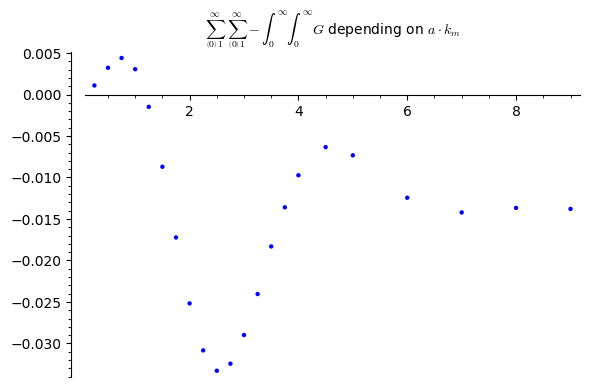
\includegraphics[width=0.46\textwidth]{sum_sum_int_int_G_on_a_km.png}
\caption{}{\centering{\textbf{Fig.2.} How $\sum\limits_{\left(0\right)\,1}^{\infty}\,\,\sum\limits_{\left(0\right)\,1}^{\infty}-\int\limits_{0}^{\infty}\int\limits_{0}^{\infty}G$ depends on $a \cdot k_m$.}}
\end{center}
\label{fig:G_on_a_km}
\end{figure}



    According to our calculation we can see that

\vspace{-3.5mm}
\begin{equation}
\begin{array}{l}
    \int\limits_{0}^{\infty} \Bigg\{ \sum\limits_{n_x=\left(0\right)\,1}^{\infty} \sum\limits_{n_y=\left(0\right)\,1}^{\infty} F\left(n_x, n_y\right) \\
- \int\limits_{0}^{\infty} \int\limits_{0}^{\infty} F\left(n_x, n_y\right) d{n_x} d{n_y} \Bigg\} d{u} \approx R\left(a k_m\right),
\end{array}
\end{equation}


    where \(R\left(a k_m\right)\) is a function depended on material
properties with well defined limit at \(a\,k_m\,»\,1\). So

    \begin{equation}
\delta\,\frac{E}{V} = R\left(a k_m\right)\,\frac{\hbar\,c\,\pi}{a^4}.
\end{equation}

    For the energy density difference per \(cm^2\) (in the limit at
\(a\,k_m\,\rightarrow \,10\)) we find that

    \(\delta\,\frac{E}{V} = \hbar\,c\, \pi\frac{R}{a^4}\,=\,0.0136\,\frac{1}{a_{\mu}^4}\,dyne/cm^2\)

    where \(a_{\mu}\) is a square side of honeycombs measured in microns.


    Can this difference of specific energy density
\(\delta\left(E/V\right)\) be interpreted as the cause of the force
\(F\) applied to perfectly conducting honeycomb on a plate? For example,
my investigations of the configuration used by Casimir have shown that for the
geometric configuration of two perfectly conducting plates
\(F/S = -3 \cdot \delta\left(E/V\right)\). But what can be said about honeycomb
configuration? Research of this question presented in appendixes B and C
shows that \(F/S \approx \delta\left(E/V\right)\).

% \end{multicols}

\vspace{\myvspacebeforesubsection}
    \subsection*{\centering{\fontencoding{T1}\fontfamily{ptm}{\selectfont CONCLUSION}}} \label{conclusions}
\vspace{\myvspaceaftersubsection}

% \begin{multicols}{2}

    Therefore, the following conclusions can be drawn: there is a force applied
to perfectly conducting honeycombs on a plate as a result of the
difference in specific energy density on its different sides. This force
depends on the material of the plate. This force depends
on the cutoff frequency \(\omega_m\) of the honeycomb plate material at least.
This force can be interpreted as the pressure of the zero-point
electromagnetic oscillations.

    Although the effect is small, an experimental confirmation seems not
unfeasible and might be of a certain interest.

    Tuo Qu, Fang Liu, Yuechai Lin, Yidong Huang \cite{Tuo2019} have reported
the production of gold nano-honeycomb with a size of about 2
microns. According to the formula presented in this work that honeycomb should
have Casimir energy density difference about
\(\delta\left(E/V\right) = 0.0136/({2^4}) = 0.0008555\,dyne/cm^2 = 0.0008555 \cdot 10^4 = 8.55\,dyne/m^2\),
that is 8.55 dynes per square meter of the panel, which is quite
an acceptable value for the practical use of the expected effect for
satellite orbits correction.

    It is important to point out, that according to the proposed method,
the \(\delta\left(E/V\right)\) is
calculated not for the total surface area of the honeycombs, but for a
part of the panel occupied by cavities (minus the area of the
honeycomb walls).

    That does not mean, the honeycomb walls should be made as thin
as possible, because with a decrease in the wall thickness, the value of
\(k_m\) will also decrease.

    For simplicity of calculations, square-shaped nanocells have been analyzed,
but the obtained result can be used, with some correction unknown so far,
to estimate the Casimir effect in honeycombs of a different shape
(hexagonal, cylindrical, etc.). Such honeycombs are simpler to be manufactured,
but require much more complex calculations to estimate the Casimir effect exactly.
In addition, the bottom of the honeycomb is not necessarily flat, but
spherically concave, for example, which does not fundamentally affect
the magnitude of the thrust.

    In addition, the appearance of Casimir thrust is expected not only in metal honeycombs,
but in dielectric honeycombs as well, because the Casimir effect in dielectrics
is well known.

    It has been assumed that the height of the the walls of the honeycombs is \(L/2\),
while the real height of the walls \(h\) will be much smaller (say about \(a\)).

    At the same time, by using the Antipin approach (see Appendix D) it can be
shown that the effect should be observed at a smaller height of the
ribs, although the dependence of the effect on the height may be the
subject of further research.

    To answer Hrvoje \cite{Hrvoje2016} who considers the Casimir
effect as not a consequence of the existence of virtual quantum photons,
but as manifestation of the London-Van der Waals dispersion
forces, I would like to note that setting up an experiment to measure the thrust
produced by nanocells grown on metal plate could serve as a critical
experiment to find out which points of view on the nature of the
Casimir force corresponds to reality.

\end{multicols}

\vspace{\myvspacebeforesubsection}
    \subsection*{\centering {\fontencoding{T1}\fontfamily{ptm}{\selectfont \uppercase{Appendix A. Integration details}}}}\label{appendix-a.-integration-details}
\vspace{\myvspaceaftersubsection}

\begin{multicols}{2}
    Let us use the regularization function in the form

\setcounter{equation}{0}
\renewcommand{\theequation}{A.\arabic{equation}}

\begin{equation}
f\left(\frac{k}{k_m}\right) = \frac{1}{\frac{k^{4}}{k_{m}^{4}} + 1}.
\end{equation}


    Starting from (\ref{eq:4}) and by introducing a variable \(n_{xy} = \sqrt{n_x^2 + n_y^2}\) and \(n = \sqrt{n_x^2 + n_y^2 + u^2} = \sqrt{n_{xy}^2 + u^2}\), we have 

\noindent
\begin{equation}
F\left(u, n_{xy}, ak_m\right) = \frac{\sqrt{n_{\mathit{xy}}^{2} + u^{2}}}{\frac{\pi^{4} {\left(n_{\mathit{xy}}^{2} + u^{2}\right)}^{2}}{\mathit{ak}_{m}^{4}} + 1}.
\end{equation}


And using this variable, we can make the following substitution

\vspace{1.5mm}
\(u = \sqrt{n^2 - n_x^2 - n_y^2} = \sqrt{n^2 - n_{xy}^2}\),
\(\frac{du}{dn} = \frac{n}{\sqrt{n^{2} - \mathit{n_{xy}}^{2}}}\), $\,\,\,\,\,\,\,\,\,$
 \(d{u}= \frac{n\,d{n}}{\sqrt{n^{2} - \mathit{n_{xy}}^{2}}}\).

    And now we can rewrite integral (\ref{eq:5}) in form

\begin{equation}
G%\left(n_x, n_y\right)
 = \int\limits_{0}^{\infty}\sqrt{n_{xy}^2+u^2}\,
f\left(\frac{\pi\sqrt{n_{xy}^2+u^2}}{a\,k_m}\right)\,d{u},
\end{equation}

changing the integration variable from \(u\) to \(n\)

\noindent
$G%\left(n_x, n_y\right)
 = \int\limits_{n_{xy}}^{\infty}\sqrt{n_{xy}^2+u^2}
 f\left(\frac{\pi\sqrt{n_{xy}^2+u^2}}{a\,k_m}\right)\,dn\,{\frac{n}{\sqrt{n^{2} - n_{xy}^{2}}}}$

\begin{equation}
G\left(n_x, n_y\right) = \int\limits_{n_{xy}}^{\infty}n\,
f\left(\frac{\pi\,n}{a\,k_m}\right)\,dn\,{\frac{n}{\sqrt{n^{2} - n_{xy}^{2}}}},
\end{equation}

    because in this form integral can be taken analytically. So, we have
the following integrand

\begin{equation} \label{eq:A5}
F\left(n, n_{xy}, ak_m\right) = \frac{n^{2}}{{\left(\frac{\pi^{4} n^{4}}{\mathit{ak}_{m}^{4}} + 1\right)} \sqrt{n^{2} - n_{\mathit{xy}}^{2}}}
\end{equation}

    and the following limits of integration by \(n\): \(n_a = n_{xy}\),
\(n_b = \infty\).

    Let us use the Abel substitution:

\begin{equation}
t = \left(\sqrt{n^2-n_{xy}^2}\right)', \,\,\,\,\,\,\,\,\,\,\, t = \frac{n}{\sqrt{n^{2} - n_{\mathit{xy}}^{2}}}
\end{equation}

    and the following limits of integration by \(t\): \(t_a = +\infty\),
\(t_b = +1\).

    Let us denote dependency of \(n\) from \(t\)

\begin{equation}
n^{2} = \frac{n_{\mathit{xy}}^{2} t^{2}}{t^{2} - 1}, \,\,\,\,\,\,\,\,\, n = n_{\mathit{xy}} \sqrt{\frac{t^{2}}{t^{2} - 1}}
\end{equation}

    and derivatives

    \[\frac{dt}{dn} = \frac{d}{dn} \left( \frac{n}{\sqrt{n^{2} - n_{\mathit{xy}}^{2}}} \right)= -\frac{n^{2}}{{\left(n^{2} - n_{\mathit{xy}}^{2}\right)}^{\frac{3}{2}}} + \frac{1}{\sqrt{n^{2} - n_{\mathit{xy}}^{2}}},\]

\begin{equation}
\frac{dn}{dt} = -\frac{n^{4} - 2 \, n^{2} n_{\mathit{xy}}^{2} + n_{\mathit{xy}}^{4}}{\sqrt{n^{2} - n_{\mathit{xy}}^{2}} n_{\mathit{xy}}^{2}}.
\end{equation}

    Now we can rewrite the integrand, making it depending on \(t\)

    \[F\left(t, n_{xy}, ak_m\right) = F\left(n, n_{xy}, ak_m\right) \cdot \frac{dn}{dt} \, \Bigg\rvert_{ n = n_{\mathit{xy}} \sqrt{\frac{t^{2}}{t^{2} - 1}} }\]

\[F\left(n, n_{xy}, ak_m\right) \cdot \frac{dn}{dt} = -\frac{{\left(n^{4} - 2 \, n^{2} n_{\mathit{xy}}^{2} + n_{\mathit{xy}}^{4}\right)} n^{2}}{{\left(\frac{\pi^{4} n^{4}}{\mathit{ak}_{m}^{4}} + 1\right)} {\left(n^{2} - n_{\mathit{xy}}^{2}\right)} n_{\mathit{xy}}^{2}}\]

\[F\left(t, n_{xy}, ak_m\right) = -\frac{{\left(\frac{n_{\mathit{xy}}^{4} t^{4}}{{\left(t^{2} - 1\right)}^{2}} - \frac{2 \, n_{\mathit{xy}}^{4} t^{2}}{t^{2} - 1} + n_{\mathit{xy}}^{4}\right)} t^{2}}{{\left(\frac{\pi^{4} n_{\mathit{xy}}^{4} t^{4}}{{\left(t^{2} - 1\right)}^{2} \mathit{ak}_{m}^{4}} + 1\right)} {\left(\frac{n_{\mathit{xy}}^{2} t^{2}}{t^{2} - 1} - n_{\mathit{xy}}^{2}\right)} {\left(t^{2} - 1\right)}}\]

\[F\left(t, n_{xy}, ak_m\right) = \frac{\mathit{ak}_{m}^{4} n_{\mathit{xy}}^{2} t^{2}}{2 \, \mathit{ak}_{m}^{4} t^{2} - {\left(\pi^{4} n_{\mathit{xy}}^{4} + \mathit{ak}_{m}^{4}\right)} t^{4} - \mathit{ak}_{m}^{4}}\]

    Let us extract coefficient near \(t^4\) from the denominator.

    Now let us move the above coefficient up to the numerator. So, the new
numerator will be

    \[-\frac{\mathit{ak}_{m}^{4} n_{\mathit{xy}}^{2} t^{2}}{\pi^{4} n_{\mathit{xy}}^{4} + \mathit{ak}_{m}^{4}}.\]

    Accordingly, the new denominator will be

    \[-\frac{2 \, \mathit{ak}_{m}^{4} t^{2}}{\pi^{4} n_{\mathit{xy}}^{4} + \mathit{ak}_{m}^{4}} + t^{4} + \frac{\mathit{ak}_{m}^{4}}{\pi^{4} n_{\mathit{xy}}^{4} + \mathit{ak}_{m}^{4}}.\]

    Now we should convert this denominator to the following form

    \[-{\left(\alpha_{1} t + t^{2} + \beta_{1}\right)} {\left(\alpha_{1} t - t^{2} - \beta_{1}\right)},\]

\[t^{4} - {\left(\alpha_{1}^{2} - 2 \, \beta_{1}\right)} t^{2} + \beta_{1}^{2}.\]

    % Begin:

    So, we have the following equation

\[-\frac{2 \, \mathit{ak}_{m}^{4} t^{2}}{\pi^{4} n_{\mathit{xy}}^{4} + \mathit{ak}_{m}^{4}} + t^{4} + \frac{\mathit{ak}_{m}^{4}}{\pi^{4} n_{\mathit{xy}}^{4} + \mathit{ak}_{m}^{4}} = t^{4} - {\left(\alpha_{1}^{2} - 2 \, \beta_{1}\right)} t^{2} + \beta_{1}^{2}\]

and its solution

\begin{equation}\beta_{1} = \frac{\mathit{ak}_{m}^{2}}{\sqrt{\pi^{4} n_{\mathit{xy}}^{4} + \mathit{ak}_{m}^{4}}},\end{equation} \begin{equation}\alpha_{1} = \sqrt{2} \mathit{ak}_{m} \sqrt{\frac{\mathit{ak}_{m}^{2} + \sqrt{\pi^{4} n_{\mathit{xy}}^{4} + \mathit{ak}_{m}^{4}}}{\pi^{4} n_{\mathit{xy}}^{4} + \mathit{ak}_{m}^{4}}}.\end{equation}

    After the conversion determined above, the integrand can be presented as

    \[\frac{\mathit{ak}_{m}^{4} n_{\mathit{xy}}^{2} t^{2}}{{\left(\pi^{4} n_{\mathit{xy}}^{4} + \mathit{ak}_{m}^{4}\right)} {\left(\alpha_{1} t + t^{2} + \beta_{1}\right)} {\left(\alpha_{1} t - t^{2} - \beta_{1}\right)}}.\]

    Let us check determinant \(\alpha_1^2 - 4\beta_1\) by using the
expression of \(\alpha_1\) and \(\beta_1\) found above.

    The determinant is negative and the integral can be easily calculated:

\noindent
    \[\begin{array}{r} \int F\left(t, n_{xy}, ak_m\right) dt = -\frac{\mathit{ak}_{m}^{4} n_{\mathit{xy}}^{2}}{4 \, {\left(\pi^{4} n_{\mathit{xy}}^{4} + \mathit{ak}_{m}^{4}\right)}} \Bigg(\frac{2 \, \arctan\left(\frac{\alpha_{1} + 2 \, t}{\sqrt{-\alpha_{1}^{2} + 4 \, \beta_{1}}}\right)}{\sqrt{-\alpha_{1}^{2} + 4 \, \beta_{1}}} + \\ \frac{2 \, \arctan\left(-\frac{\alpha_{1} - 2 \, t}{\sqrt{-\alpha_{1}^{2} + 4 \, \beta_{1}}}\right)}{\sqrt{-\alpha_{1}^{2} + 4 \, \beta_{1}}} - \frac{\log\left(\alpha_{1} t + t^{2} + \beta_{1}\right)}{\alpha_{1}} + \frac{\log\left(-\alpha_{1} t + t^{2} + \beta_{1}\right)}{\alpha_{1}}\Bigg). \end{array}\]

%    And after substitution of \(t\) value
% \(\int F\left(n, n_{xy}, ak_m\right) dn\) is:

%    \(\begin{array}{r} \int F\left(n, n_{xy}, ak_m\right) dn = -\frac{\mathit{ak}_{m}^{4} n_{\mathit{xy}}^{2}}{4 \, {\left(\pi^{4} n_{\mathit{xy}}^{4} + \mathit{ak}_{m}^{4}\right)}} \Bigg(\frac{2 \, \arctan\left(\frac{\alpha_{1} + \frac{2 \, n}{\sqrt{n^{2} - n_{\mathit{xy}}^{2}}}}{\sqrt{-\alpha_{1}^{2} + 4 \, \beta_{1}}}\right)}{\sqrt{-\alpha_{1}^{2} + 4 \, \beta_{1}}} + \\ \frac{2 \, \arctan\left(-\frac{\alpha_{1} - \frac{2 \, n}{\sqrt{n^{2} - n_{\mathit{xy}}^{2}}}}{\sqrt{-\alpha_{1}^{2} + 4 \, \beta_{1}}}\right)}{\sqrt{-\alpha_{1}^{2} + 4 \, \beta_{1}}} - \frac{\log\left(\frac{\alpha_{1} n}{\sqrt{n^{2} - n_{\mathit{xy}}^{2}}} + \beta_{1} + \frac{n^{2}}{n^{2} - n_{\mathit{xy}}^{2}}\right)}{\alpha_{1}} + \frac{\log\left(-\frac{\alpha_{1} n}{\sqrt{n^{2} - n_{\mathit{xy}}^{2}}} + \beta_{1} + \frac{n^{2}}{n^{2} - n_{\mathit{xy}}^{2}}\right)}{\alpha_{1}}\Bigg) \end{array}\)

%    Checking that found integral is true by differentiation:

%     \[\left( \int F\left(n, n_{xy}, ak_m\right) dn \right)' = \frac{\sqrt{n^{2} - n_{\mathit{xy}}^{2}} \mathit{ak}_{m}^{4} n^{2}}{\pi^{4} n^{6} + \mathit{ak}_{m}^{4} n^{2} - {\left(\pi^{4} n^{4} + %  % \mathit{ak}_{m}^{4}\right)} n_{\mathit{xy}}^{2}}\]

% \[F\left(n, n_{xy}, ak_m\right)= \frac{n^{2}}{{\left(\frac{\pi^{4} n^{4}}{\mathit{ak}_{m}^{4}} + 1\right)} \sqrt{n^{2} - n_{\mathit{xy}}^{2}}}\]

% \[\left( \int F\left(n, n_{xy}, ak_m\right) dn \right)'-F\left(n, n_{xy}, ak_m\right) = 0\]

%    So, we received true expression of integral
% \(\int F\left(n, n_{xy}, ak_m\right) dn\)

% Now using its \(t_a\) and \(t_b\) limits we found the following
% integral:

    % \(\begin{array}{r}  G\left(n_{xy}\right) = \int\limits_{0}^{\infty}\sqrt{n_{xy}^2+u^2}\, f\left(\frac{\pi\sqrt{n_{xy}^2+u^2}}{a\,k_m}\right)\,d{u} = \\  -\frac{\mathit{ak}_{m}^{4} n_{\mathit{xy}}^{2} {\left(\frac{2 \, \arctan\left(\frac{\alpha_{1} + 2}{\sqrt{-\alpha_{1}^{2} + 4 \, \beta_{1}}}\right)}{\sqrt{-\alpha_{1}^{2} + 4 \, \beta_{1}}} + \frac{2 \, \arctan\left(-\frac{\alpha_{1} - 2}{\sqrt{-\alpha_{1}^{2} + 4 \, \beta_{1}}}\right)}{\sqrt{-\alpha_{1}^{2} + 4 \, \beta_{1}}} - \frac{\log\left(\alpha_{1} + \beta_{1} + 1\right)}{\alpha_{1}} + \frac{\log\left(-\alpha_{1} + \beta_{1} + 1\right)}{\alpha_{1}}\right)}}{4 \, {\left(\pi^{4} n_{\mathit{xy}}^{4} + \mathit{ak}_{m}^{4}\right)}} \\ +\frac{\pi \mathit{ak}_{m}^{4} n_{\mathit{xy}}^{2}}{2 \, {\left(\pi^{4} \sqrt{-\alpha_{1}^{2} + 4 \, \beta_{1}} n_{\mathit{xy}}^{4} + \sqrt{-\alpha_{1}^{2} + 4 \, \beta_{1}} \mathit{ak}_{m}^{4}\right)}} \end{array}\)


\end{multicols}

\pagebreak

\vspace{\myvspacebeforesubsection}
    \subsection*{\centering {\fontencoding{T1}\fontfamily{ptm}{\selectfont \uppercase{Appendix B. Electromagnetic pressure
calculation}}}} \label{appendix-b.-electromagnetic-pressure-calculation}
\vspace{\myvspaceaftersubsection}

\begin{multicols}{2}

\setcounter{equation}{0}
\renewcommand{\theequation}{B.\arabic{equation}}

    Let us consider a rectangular resonator with size \(a \times b \times h\).

    \textbf{For the electric mode}

\begin{equation}\nabla\,\vec{E} + \frac{\omega^2}{c^2}\,\vec{E} = 0,\end{equation} we have the
following solution

\[E_{x} = A_{x} \cos\left(\frac{\pi n_{x} x}{a}\right) \sin\left(\frac{\pi n_{y} y}{b}\right) \sin\left(k_{z} z\right)\]
\[E_{y} = A_{y} \cos\left(\frac{\pi n_{y} y}{b}\right) \sin\left(\frac{\pi n_{x} x}{a}\right) \sin\left(k_{z} z\right)\]
\[E_{z} = A_{z} \cos\left(k_{z} z\right) \sin\left(\frac{\pi n_{x} x}{a}\right) \sin\left(\frac{\pi n_{y} y}{b}\right)\]

and

\[H_{x} = \frac{i \, {\left(A_{y} b k_{z} - \pi A_{z} n_{y}\right)} c \cos\left(\frac{\pi n_{y} y}{b}\right) \cos\left(k_{z} z\right) \sin\left(\frac{\pi n_{x} x}{a}\right)}{b \mu \omega}\]
\[H_{y} = -\frac{i \, {\left(A_{x} k_{z} - \frac{\pi A_{z} n_{x}}{a}\right)} c \cos\left(\frac{\pi n_{x} x}{a}\right) \cos\left(k_{z} z\right) \sin\left(\frac{\pi n_{y} y}{b}\right)}{\mu \omega}\]
\[H_{z} = -\frac{i \, {\left(\frac{\pi A_{y} n_{x}}{a} - \frac{\pi A_{x} n_{y}}{b}\right)} c \cos\left(\frac{\pi n_{x} x}{a}\right) \cos\left(\frac{\pi n_{y} y}{b}\right) \sin\left(k_{z} z\right)}{\mu \omega}\]

with

\begin{equation}k_{z}^{2} + \frac{\pi^{2} n_{x}^{2}}{a^{2}} + \frac{\pi^{2} n_{y}^{2}}{b^{2}} - \frac{\omega^{2}}{c^{2}} = 0,\end{equation}

by using \(div\,\vec{E} = 0\), we have

\begin{equation}A_{z} k_{z} + \frac{\pi A_{x} n_{x}}{a} + \frac{\pi A_{y} n_{y}}{b} = 0.\end{equation}

Field energy density
\(\left(\int \frac{E_x^2+E_y^2+E_z^2}{8 \pi}dV\right)\big/{V}\) is

\begin{equation}\frac{E}{V} = \frac{{A_{x}^{2} + A_{y}^{2} + A_{z}^{2}} }{64 \, \pi}.\end{equation}

    Full energy density
% \(\left(\int \frac{E_x^2+E_y^2+E_z^2}{8 \pi}dV + \int \frac{H_x^2+H_y^2+H_z^2}{8 \pi}dV\right)\big/{V}\)
\(\left(\int \frac{|\vec{E}|^2}{8 \pi}dV + \int \frac{|\vec{H}|^2}{8 \pi}dV\right)\big/{V}\)
is

\begin{equation}\frac{E}{V} = \frac{{A_{x}^{2} + A_{y}^{2} + A_{z}^{2}}}{32 \, \pi}.\end{equation}

    Electromagnetic pressure
\(\left({\int \frac {H_x^2+H_y^2}{8 \pi} dS}\right)\big/{S}\) on \(xy\)
plate is

\end{multicols}

% \renewcommand{\theequation}{B.\arabic{equation}}

\begin{equation}\frac{f_z}{S} = -\frac{2 \, \pi A_{x} A_{z} a b^{2} k_{z} n_{x} - \pi^{2} A_{z}^{2} b^{2} n_{x}^{2} + 2 \, \pi A_{y} A_{z} a^{2} b k_{z} n_{y} - \pi^{2} A_{z}^{2} a^{2} n_{y}^{2} - {\left(A_{x}^{2} + A_{y}^{2}\right)} a^{2} b^{2} k_{z}^{2}}{32 \, {\left(\pi a^{2} b^{2} k_{z}^{2} + \pi^{3} b^{2} n_{x}^{2} + \pi^{3} a^{2} n_{y}^{2}\right)}}.\end{equation}

    Their relation \(\frac{f_z/S}{E/V}\) is

\begin{equation}\frac{f_z/S}{E/V} = \frac{A_{x}^{2} a^{2} b^{2} k_{z}^{2} + A_{y}^{2} a^{2} b^{2} k_{z}^{2} - 2 \, \pi A_{x} A_{z} a b^{2} k_{z} n_{x} + \pi^{2} A_{z}^{2} b^{2} n_{x}^{2} - 2 \, \pi A_{y} A_{z} a^{2} b k_{z} n_{y} + \pi^{2} A_{z}^{2} a^{2} n_{y}^{2}}{{\left(a^{2} b^{2} k_{z}^{2} + \pi^{2} b^{2} n_{x}^{2} + \pi^{2} a^{2} n_{y}^{2}\right)} {\left(A_{x}^{2} + A_{y}^{2} + A_{z}^{2}\right)}}.\end{equation}

\begin{multicols}{2}

    Considering solution with wave propagation in \(z\)-direction we have
\(H_z = 0\) which gives

    \[\pi A_{y} b n_{x} - \pi A_{x} a n_{y} = 0\]

    and

\[A_{x} = -\frac{A_{z} a b^{2} k_{z} n_{x}}{\pi b^{2} n_{x}^{2} + \pi a^{2} n_{y}^{2}},
A_{y} = -\frac{A_{z} a^{2} b k_{z} n_{y}}{\pi b^{2} n_{x}^{2} + \pi a^{2} n_{y}^{2}}.\]

    In this case the relation of electromagnetic pressure per field energy density
is equal to \(1\),

\begin{equation}\frac{f_z/S}{E/V} = 1.\end{equation}

    Considering solution with wave propagation in \(x\)-direction we have
\(H_x = 0\) which gives

    \[A_{y} = -\frac{\pi^{2} A_{x} b n_{x} n_{y}}{a b^{2} k_{z}^{2} + \pi^{2} a n_{y}^{2}},
A_{z} = -\frac{\pi A_{x} b^{2} k_{z} n_{x}}{a b^{2} k_{z}^{2} + \pi^{2} a n_{y}^{2}}.\]

    In this case the relation of electromagnetic pressure per field energy density is

\begin{equation}\frac{f_z/S}{E/V} = \frac{b^{2} k_{z}^{2}}{b^{2} k_{z}^{2} + \pi^{2} n_{y}^{2}}.\end{equation}

    Considering solution with wave propagation in \(y\)-direction,
\(H_y = 0\), as in \(x\)-direction

\[A_{x} = -\frac{\pi^{2} A_{y} a n_{x} n_{y}}{a^{2} b k_{z}^{2} + \pi^{2} b n_{x}^{2}},
A_{z} = -\frac{\pi A_{y} a^{2} k_{z} n_{y}}{a^{2} b k_{z}^{2} + \pi^{2} b n_{x}^{2}},\]

\begin{equation}\frac{f_z/S}{E/V} = \frac{a^{2} k_{z}^{2}}{a^{2} k_{z}^{2} + \pi^{2} n_{x}^{2}}.\end{equation}

    \textbf{For the magnetic mode}

\begin{equation}\nabla\,\vec{H} + \frac{\omega^2}{c^2}\,\vec{H} = 0\end{equation}, we have the
following solution

    \[H_{x} = B_{1} \cos\left(\frac{\pi n_{y} y}{b}\right) \cos\left(k_{z} z\right) \sin\left(\frac{\pi n_{x} x}{a}\right)\]
\[H_{y} = B_{2} \cos\left(\frac{\pi n_{x} x}{a}\right) \cos\left(k_{z} z\right) \sin\left(\frac{\pi n_{y} y}{b}\right)\]
\[H_{z} = B_{3} \cos\left(\frac{\pi n_{x} x}{a}\right) \cos\left(\frac{\pi n_{y} y}{b}\right) \sin\left(k_{z} z\right)\]

    and

\[E_{x} = \frac{i \, {\left(B_{2} k_{z} - \frac{\pi B_{3} n_{y}}{b}\right)} c \cos\left(\frac{\pi n_{x} x}{a}\right) \sin\left(\frac{\pi n_{y} y}{b}\right) \sin\left(k_{z} z\right)}{\mu \omega}\]
\[E_{y} = -\frac{i \, {\left(B_{1} k_{z} - \frac{\pi B_{3} n_{x}}{a}\right)} c \cos\left(\frac{\pi n_{y} y}{b}\right) \sin\left(\frac{\pi n_{x} x}{a}\right) \sin\left(k_{z} z\right)}{\mu \omega}\]
\[E_{z} = -\frac{i \, {\left(\frac{\pi B_{2} n_{x}}{a} - \frac{\pi B_{1} n_{y}}{b}\right)} c \cos\left(k_{z} z\right) \sin\left(\frac{\pi n_{x} x}{a}\right) \sin\left(\frac{\pi n_{y} y}{b}\right)}{\mu \omega}\]

    with

\begin{equation}k_{z}^{2} + \frac{\pi^{2} n_{x}^{2}}{a^{2}} + \frac{\pi^{2} n_{y}^{2}}{b^{2}} - \frac{\omega^{2}}{c^{2}} = 0,\end{equation}

    by using \(div\,\vec{H} = 0\), we have

\begin{equation}B_{3} k_{z} + \frac{\pi B_{1} n_{x}}{a} + \frac{\pi B_{2} n_{y}}{b} = 0.\end{equation}

    Magnetic field energy density
\(\left(\int \frac{H_x^2+H_y^2+H_z^2}{8 \pi}dV\right)\big/{V}\) is

\begin{equation}\frac{E}{V} = \frac{{B_{1}^{2} + B_{2}^{2} + B_{3}^{2}}}{64 \, \pi}.\end{equation}

    Full energy density
\(\left(\int \frac{|\vec{E}|^2}{8 \pi}dV + \int \frac{|\vec{H}|^2}{8 \pi}dV\right)\big/{V}\)
is

\begin{equation}\frac{E}{V} = \frac{{B_{1}^{2} + B_{2}^{2} + B_{3}^{2}}}{32 \, \pi}.\end{equation}

    Electromagnetic pressure
\(\left({\int \frac {H_x^2+H_y^2}{8 \pi} dS}\right)\big/{S}\) on \(xy\)
plate is

\begin{equation}\frac{f_z}{S}=\frac{{B_{1}^{2} + B_{2}^{2}}}{32 \, \pi}.\end{equation}

Their relation \(\frac{f_z/S}{E/V}\) is

\begin{equation}\frac{f_z/S}{E/V} = \frac{{B_{1}^{2} + B_{2}^{2}}}{B_{1}^{2} + B_{2}^{2} + B_{3}^{2}}.\end{equation}

Considering solution with wave propagation in \(z\)-direction, we have
\(E_z = 0\) which gives

\[\frac{\pi B_{2} n_{x}}{a} - \frac{\pi B_{1} n_{y}}{a} = 0\]

and

\[B_1 = -\frac{B_{3} a k_{z} n_{x}}{\pi n_{x}^{2} + \pi n_{y}^{2}},
B_2 = -\frac{B_{3} a k_{z} n_{y}}{\pi n_{x}^{2} + \pi n_{y}^{2}}.\]

In this case the relation of electromagnetic pressure per field energy density is

\begin{equation}\frac{f_z/S}{E/V} = \frac{a^{2} k_{z}^{2}}{a^{2} k_{z}^{2} + \pi^{2} n_{x}^{2} + \pi^{2} n_{y}^{2}}.\end{equation}

    Considering solution with wave propagation in \(x\)-direction, we have
\(E_x = 0\) which gives

\[B_2 = -\frac{\pi^{2} B_{1} n_{x} n_{y}}{a^{2} k_{z}^{2} + \pi^{2} n_{y}^{2}},
B_3 = -\frac{\pi B_{1} a k_{z} n_{x}}{a^{2} k_{z}^{2} + \pi^{2} n_{y}^{2}}.\]

In this case the relation of electromagnetic pressure per field energy density is

\[\frac{f_z/S}{E/V} = \frac{a^{2} b^{4} k_{z}^{4} + 2 \, \pi^{2} a^{2} b^{2} k_{z}^{2} n_{y}^{2} + \pi^{4} b^{2} n_{x}^{2} n_{y}^{2} + \pi^{4} a^{2} n_{y}^{4}}{{\left(a^{2} b^{2} k_{z}^{2} + \pi^{2} b^{2} n_{x}^{2} + \pi^{2} a^{2} n_{y}^{2}\right)} {\left(b^{2} k_{z}^{2} + \pi^{2} n_{y}^{2}\right)}}.\]

Considering solution with wave propagation in \(y\)-direction
\(E_y = 0\) as in \(x\)-direction

    \[B_1 = -\frac{\pi^{2} B_{2} n_{x} n_{y}}{a^{2} k_{z}^{2} + \pi^{2} n_{x}^{2}},
      B_3 = -\frac{\pi B_{2} a k_{z} n_{y}}{a^{2} k_{z}^{2} + \pi^{2} n_{x}^{2}},\]

\[\frac{f_z/S}{E/V} = \frac{a^{4} b^{2} k_{z}^{4} + 2 \, \pi^{2} a^{2} b^{2} k_{z}^{2} n_{x}^{2} + \pi^{4} b^{2} n_{x}^{4} + \pi^{4} a^{2} n_{x}^{2} n_{y}^{2}}{{\left(a^{2} b^{2} k_{z}^{2} + \pi^{2} b^{2} n_{x}^{2} + \pi^{2} a^{2} n_{y}^{2}\right)} {\left(a^{2} k_{z}^{2} + \pi^{2} n_{x}^{2}\right)}}.\]

    So, we can see that task of electromagnetic force calculation in the
nanohoneycomb configuration is quit easy, because

\begin{equation}\lim_{k_z \to \infty}\frac{f_z/S}{E/V} = 1.\end{equation}

We can see that if we decrease \(a\) then \(\frac{f_z/S}{E/V}\) also decreases
and that leads to

\begin{equation}\frac{F}{S} \geq \delta\,\frac{E}{V} = \hbar\,c\, \pi\frac{R}{a^4}.\end{equation}

On the other hand, the same result can be shown by using
Hamiltonian mechanics approach.

% \end{multicols}

\vspace{\myvspacebeforesubsection}
    \subsection*{\centering {\fontencoding{T1}\fontfamily{ptm}{\selectfont \uppercase{Appendix C. Hamiltonian mechanics
approach}}}} \label{appendix-c.-hamiltonian-mechanics-approach}
\vspace{\myvspaceaftersubsection}

% \begin{multicols}{2}

\setcounter{equation}{0}
\renewcommand{\theequation}{C.\arabic{equation}}

    Let us consider a cubic cavity of volume \(L^3\) bounded by perfectly
conducting walls where perfectly conducting square plate with side
\(L\) is placed in this cavity parallel to the \(xy\) face, and let the distance
between the plate and \(xy\) face be sufficiently large, say \(l = L/2\), for example.

One side of this perfectly conducting square plate is a smooth plane and
another is covered by perfectly conducting square-shaped honeycomb a square side \(a\).

On both sided of the the plate the expressions \(1\big/2\sum\,\hbar\omega\)
where the summation extends over all possible resonance frequencies of
the cavity \(\left(L-l\right)\times L\times L\) (a large cavity between
smooth plane and \(xy\) face) and the cavity \(l\times a\times a\) (a small
cavity, one honeycomb cell) are divergent and devoid of physical meaning,
but it will be shown that for the both
opposite sides the derivative \({d\left<0|\hat{\mathcal{H}}|0\right>}\big/{dl}\) of
the vacuums Hamiltonian of the whole system for these sums
\(\left<0|\hat{\mathcal{H}}|0\right> = 1\big/2\,\left(\sum\,\,\hbar\omega\right)_{I} + 1\big/2\,\left(\sum\,\,\hbar\omega\right)_{II}\),
has a well-defined value and this value will be
interpreted as the interaction between the plate and the both \(xy\) faces.

\begin{figure}
\begin{center}
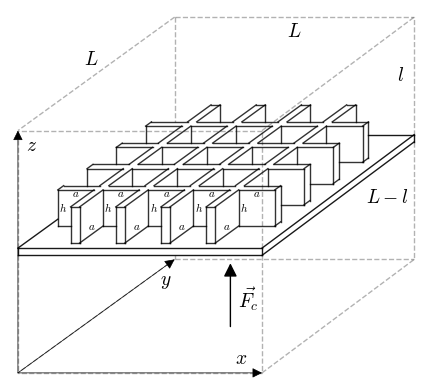
\includegraphics[width=0.42\textwidth]{honeycomb_box_H.png}
\caption{}{\centering{\textbf{Fig.3.} Cubic cavity with a plate covered by honeycomb.}}
\end{center}
\label{fig:honeycomb_box_H}
\end{figure}

    The possible oscillations of the cavities defined by
\(0 \leq x \leq L\), \(0 \leq y \leq L\), \(0 \geq z \geq -\,(L-l)\) (a large cavity between smooth
plane and \(xy\) face)
and
\(0 \leq x \leq a\), \(0 \leq y \leq a\), \(0 \leq z \leq l\) (a small cavity, one honeycomb cell)
    have the wave vectors
\(k_x = \frac{\pi}{L}\,n_x\), \(k_y = \frac{\pi}{L}\,n_y\),
\(k_z = \frac{\pi}{L-l}\,n_z\) (a large cavity between smooth plane and
\(xy\) face),
and
\(k_x = \frac{\pi}{a}\,n_x\), \(k_y = \frac{\pi}{a}\,n_y\),
\(k_z = \frac{\pi}{l}\,n_z\) (a small cavity, one honeycomb cell),
where \(n_x\). \(n_y\), \(n_z\) are positive integers;
\(k = \sqrt{k_x^2+k_y^2+k_z^2} = \sqrt{\kappa^2+k_z^2}\).

Let us write the expression for the sum of zero-point energy in general form

\begin{equation}
E = \frac{1}{2}\sum\,\hbar\omega = \hbar\,c\frac{1}{2}\sum\limits_{n_x}^{}\sum\limits_{n_y}^{}\sum\limits_{n_z}^{}k.
\end{equation}

    Two standing waves correspond to every \(k_x\), \(k_y\), \(k_z\), but in case when
one of the \(n_i\) is zero, there is only one wave. That is of no importance
in case of one honeycomb cell cavity for \(k_z\),
since for very large \(l\) we may regard \(k_z\) as
continuous variable, replacing summation over \(n_z\) with integration.
Thus, for a small cavity consisting of one honeycomb, we find

\noindent
\(E = \frac{\hbar c}{2}\int\limits_{0}^{\infty}\left[{\sqrt{k_z^2}+2\sum\limits_{n_x=1}^{\infty}\sum\limits_{n_y=1}^{\infty}\sqrt{\frac{n_x^2\pi^2}{a^2}+\frac{n_y^2\pi^2}{a^2}+k_z^2}}\right]d{n_z}\).

    Considering \(dn_z = \frac{l}{\pi}\,dk_z\) we can find the specific energy density \(E/S\), where
\(S = S_{small} = a^2\):

\noindent
    \(\frac{E}{S} = \frac{\hbar c}{a^2}\int\limits_{0}^{\infty}\left[{\frac{\sqrt{k_z^2}}{2}+\sum\limits_{n_x=1}^{\infty}\sum\limits_{n_y=1}^{\infty}\sqrt{\frac{n_x^2\pi^2}{a^2}+\frac{n_y^2\pi^2}{a^2}+k_z^2}}\right]\frac{l}{\pi}dk_z\),

\noindent
    \(\frac{E}{S} = \frac{\hbar c l}{a^2 \pi} \sum\limits_{n_x=(0)1}^{\infty}
\sum\limits_{n_y=(0)1}^{\infty}\Bigg[\int\limits_{0}^{\infty}\sqrt{\frac{n_x^2\pi^2}{a^2}+\frac{n_y^2\pi^2}{a^2}+k_z^2}\,dk_z\Bigg]\).

    That is of no importance in case of a large cavity for \(k_x\), \(k_y\)
since for very large \(L\) we may regard \(k_x\), \(k_y\) as
continuous variables. Thus, for large cavity between smooth plane and \(xy\) face we find
\noindent
\begin{equation}\begin{array}{l}
\begin{array}{ll}
\sum\frac{\hbar\omega}{2} = \frac{\hbar c}{2}\int\limits_{0}^{\infty}\int\limits_{0}^{\infty}\Bigg[\sqrt{k_x^2+k_y^2}\,+ & \,\\
\end{array} \\
\begin{array}{rr}
\,\,\,\,\,\,\,\,\,\,\,+ & 2\sum\limits_{n_z=1}^{\infty}\sqrt{\frac{n_z^2 \pi^2}{(L-l)^2}+k_x^2+k_y^2}\Bigg]d{n_x}d{n_y}.\end{array}
\end{array}\end{equation}

%\(\sum\frac{\hbar\omega}{2} = \frac{\hbar c}{2}\int\limits_{0}^{\infty}\int\limits_{0}^{\infty}\left[{\sqrt{k_x^2+k_y^2}+ \\
%2\sum\limits_{n_z=1}^{\infty}\sqrt{\frac{n_z^2 \pi^2}{(L-l)^2}+k_x^2+k_y^2}}\right]d{n_x}d{n_y}\)
% (large cavity between pure plane and \(xy\) face),

For very large \(L-l\) the last summation may be replaced by an
integral and, therefore, it can be seen that energy of a large cavity is given by
\noindent
\begin{equation}\sum\frac{\hbar\omega}{2} = \hbar\,c\int\limits_{0}^{\infty}\int\limits_{0}^{\infty}\int\limits_{0}^{\infty}\sqrt{k_z^2+k_x^2+k_y^2}\,d{n_x}\,d{n_y}\,d{n_z},\end{equation}
% (large cavity between pure plane and \(xy\) face),

where \(dn_x = \frac{L}{\pi}\,dk_x\), \(dn_y = \frac{L}{\pi}\,dk_y\),
\(dn_z = \frac{L-l}{\pi}\,dk_z\).

    Now for the specific (per area) energy density \(E/S\) for a large cavity, where
\(S = S_{large} = L^2\) we can write the following sequence of transformations:

\noindent
\(\frac{\sum\hbar\omega}{2 S} = \frac{\hbar\,c}{L^2}\int\limits_{0}^{\infty}\int\limits_{0}^{\infty}\int\limits_{0}^{\infty}\sqrt{k_z^2+k_x^2+k_y^2}\,dn_x\,dn_y\,\frac{L-l}{\pi}\,dk_z\),
% (large cavity between pure plane and \(xy\) face),

%\noindent
%\(\frac{\sum\hbar\omega}{2 S} = \frac{L-l}{L^2\,\pi}\hbar\,c\int\limits_{0}^{\infty}\int\limits_{0}^{\infty}\left[\,\int\limits_{0}^{\infty}\sqrt{k_z^2+k_x^2+k_y^2}\,dk_z\right]\,dn_x\,dn_y\),
% (large cavity between pure plane and \(xy\) face),

\noindent
\(\frac{E}{S} = \frac{L-l}{L^2\,\pi}\hbar\,c\int\limits_{0}^{\infty}\int\limits_{0}^{\infty}\left[\,\int\limits_{0}^{\infty}\sqrt{k_x^2+k_y^2+k_z^2}\,dk_z\right] \left(\frac{L}{\pi}dk_x\right) \left(\frac{L}{\pi}dk_y\right)\),
% (large cavity between pure plane and \(xy\) face),

\noindent
\(\frac{E}{S} = \frac{L-l}{a^2\,\pi}\hbar\,c\int\limits_{0}^{\infty}\int\limits_{0}^{\infty}\left[\,\int\limits_{0}^{\infty}\sqrt{k_x^2+k_y^2+k_z^2}\,dk_z\right] \left(\frac{a}{\pi}dk_x\right) \left(\frac{a}{\pi}dk_y\right)\).
% (large cavity between pure plane and \(xy\) face).

    Therefore, it can be seen that specific (per area) vacuum Hamiltonian
\(\frac{\left<0|\hat{\mathcal{H}}|0\right>}{S}\) of the whole system is
given by

\end{multicols}

% \noindent
% \[\begin{array}{lr}
% % \frac{\left<0|\hat{\mathcal{H}}|0\right>}{S} =
% \begin{array}{l}
% \frac{\left<0|\hat{\mathcal{H}}|0\right>}{S} = \frac{\hbar\,c}{a^2\,\pi} \cdot\\
% \cdot \Bigg\{l\sum\limits_{n_x=(0)1}^{\infty}\sum\limits_{n_y=(0)1}^{\infty}%\left[\,\int\limits_{0}^{\infty}\sqrt{n_x^2\frac{\pi^2}{a^2}+n_y^2\frac{\pi^2}{a^2}+k_z^2}\,dk_z\right] + \\
% (L-l)\int\limits_{0}^{\infty}\int\limits_{0}^{\infty}\left[\,\int\limits_{0}^{\infty}\sqrt{k_x^2+k_y^2+k_z^2}\,dk_z\right]\,\left(\frac{a}{\pi}dk_x\right)\,\left(\frac{a}{\pi}dk_y\right)\Bigg\}
% \end{array}\end{array}\]

\noindent
\[
\frac{\left<0|\hat{\mathcal{H}}|0\right>}{S} = \frac{\hbar\,c}{a^2\,\pi}
\cdot \Bigg\{l\sum\limits_{n_x=(0)1}^{\infty}\sum\limits_{n_y=(0)1}^{\infty}\left[\,\int\limits_{0}^{\infty}\sqrt{n_x^2\frac{\pi^2}{a^2}+n_y^2\frac{\pi^2}{a^2}+k_z^2}\,dk_z\right] +
(L-l)\int\limits_{0}^{\infty}\int\limits_{0}^{\infty}\left[\,\int\limits_{0}^{\infty}\sqrt{k_x^2+k_y^2+k_z^2}\,dk_z\right]\,\left(\frac{a}{\pi}dk_x\right)\,\left(\frac{a}{\pi}dk_y\right)\Bigg\}
\]

and interaction
\(\frac{F}{S} = -\frac{\partial }{\partial z} \,\frac{\left<0|\hat{\mathcal{H}}|0\right>}{S} = \frac{\partial}{\partial l} \,\frac{\left<0|\hat{\mathcal{H}}|0\right>}{S}\)
is

%\(\begin{array}{lr}\frac{F}{S} =
%\begin{array}{c}\frac{\hbar\,c}{a^2\,\pi}\Bigg\{\sum\limits_{n_x=(0)1}^{\infty}\sum\limits_{n_y=(0)1}^{\infty}\left[\,\int\limits_{0}^{\infty}\sqrt{n_x^2\frac{\pi^2}{a^2}+n_y^2\frac{\pi^2}{a^2}+k_z^2}\,dk_z\right] - \\
%\int\limits_{0}^{\infty}\int\limits_{0}^{\infty}\left[\,\int\limits_{0}^{\infty}\sqrt{k_x^2+k_y^2+k_z^2}\,dk_z\right]\,dn_x\,dn_y\Bigg\}\end{array}\end{array}\)

\noindent
\begin{equation}\frac{F}{S} = \frac{\hbar\,c}{a^2\,\pi}\left\{\sum\limits_{n_x=(0)1}^{\infty}\sum\limits_{n_y=(0)1}^{\infty}\left[\,\int\limits_{0}^{\infty}\sqrt{n_x^2\frac{\pi^2}{a^2}+n_y^2\frac{\pi^2}{a^2}+k_z^2}\,dk_z\right] -
\int\limits_{0}^{\infty}\int\limits_{0}^{\infty}\left[\,\int\limits_{0}^{\infty}\sqrt{k_x^2+k_y^2+k_z^2}\,dk_z\right]\,dn_x\,dn_y\right\}\end{equation}

\begin{multicols}{2}

    Then, the formula for the force acting on a
perfectly conducting honeycomb on a plate \({F}/{S}\) obtained by using Hamiltonian mechanics approach is the same as formula (\ref{eq:2})
received for the difference of specific energy density on its
different sides \(\delta\left({E}/{V}\right)\).

%    \begin{wrapfigure}{r}{0.5\textwidth}
%\begin{center}
%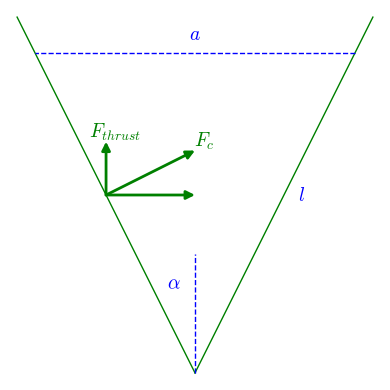
\includegraphics[width=0.48\textwidth]{Antipins_angle_en.png}
%\caption{}{Antipin's angle}
%\end{center}
%\label{fig:Antipins_angle}
%\end{wrapfigure}



\end{multicols}
\begin{multicols}{2}

\vspace{\myvspacebeforesubsection}
    \subsection*{\centering {\fontencoding{T1}\fontfamily{ptm}{\selectfont \uppercase{Appendix D. The derivation of the thrust formula for the
honeycomb basing on the Antipin's formula for the metal
angle}}}} \label{appendix-d.-the-derivation-of-the-thrust-formula-for-the-honeycomb-basing-on-the-antipin-formula-for-the-thrust-of-a-metal-angle}
\vspace{\myvspaceaftersubsection}

\setcounter{equation}{0}
\renewcommand{\theequation}{D.\arabic{equation}}

    Antipin \cite{Antipin2012} gives an estimated calculation of the thrust
of the  \mbox{V-shaped} angle by using the Casimir formula, ``with the most
general and natural approximations known as PFA (Proximity Force
Approximation) or PAA (Pairwise Additive Approximation) calculation
method \cite{Intravaia2013}, \cite{Rodriguez2011}".

\begin{figure}
\begin{center}
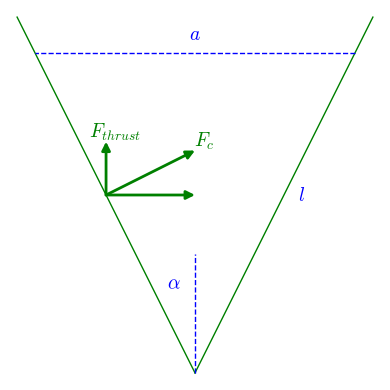
\includegraphics[width=0.45\textwidth]{Antipins_angle_en.png}
\caption{}{\centering{\textbf{Fig.4.} Antipin's angle.}}
\end{center}
\label{fig:Antipins_angle}
\end{figure}


Casimir's interaction energy is given by
\noindent
\begin{equation}\delta\,E/L^2 = \hbar\,c\frac{\pi^2}{4\,a^3}\left\{\frac{-4}{24\times30}\right\}.\end{equation}

Casimir's force is
\noindent
\begin{equation}F_{c} = \hbar\,c\frac{-3\,\pi^2}{4\,a^4}\left\{\frac{-4}{24\times30}\right\}.\end{equation}

Thrust of the metal \mbox{V-shaped} angle is
\noindent
\begin{equation}F_{thrust} = 2 \int F_{c} \, sin\, \alpha \,dS, \,\,\,\,\,\,\, dS = b\,dz\end{equation}

\noindent
\begin{equation}F_{thrust} = 2\, \frac{-3\,\pi^2\hbar c b}{4}\int\limits_{z_{min}}^{z_{max}} \left\{\frac{-4}{24\times30}\right\}\frac{sin\, \alpha\,dz}{\left(a\left(z\right)\right)^4}.\end{equation}

Let us make a substitution

\[a\left(z\right) = 2\,z\,tg\, \alpha,\]

\[F_{thrust} = 2\, \frac{-3\,\pi^2\hbar c b}{4}\int\limits_{z_{min}}^{z_{max}} \left\{\frac{-4}{24\times30}\right\}\frac{sin\, \alpha\,dz}{\left(2\,z\,tg \alpha\right)^4},\]

\[F_{thrust} = 2\, \frac{-3\,\pi^2\hbar c b}{4} \frac{sin\, \alpha}{\left(2\,tg\, \alpha\right)^4} \int\limits_{z_{min}}^{z_{max}} \left\{\frac{-4}{24\times30}\right\} \frac{dz}{z^4},\]

\[F_{thrust} = -2\cdot3\, \frac{\pi^2\hbar c b}{240} \frac{sin\, \alpha}{\left(2\,tg\, \alpha\right)^4} \left(\frac{1}{z^3}\right)\Bigg\rvert_{\,z_{min}.}^{\,z_{max}} \]

    The following substitution can be made: \[z = l\, cos\, \alpha,\]

\[F_{thrust} = -2\cdot3\, \frac{\pi^2\hbar c b}{240} \frac{sin\, \alpha}{2^4\left(tg\,\alpha\right)^4\left(cos\, \alpha\right)^3} \left(\frac{1}{l^3}\right)\Bigg\rvert_{\,l_{min},}^{\,l_{max}} \]

\[F_{thrust} = -2\cdot3\, \frac{\pi^2\hbar c b}{240} \frac{cos\, \alpha}{2^4\left(sin\, \alpha\right)^4} \left(\frac{1}{l^3}\right)\Bigg\rvert_{\,l_{min},}^{\,l_{max}} \]

\noindent
\begin{equation}F_{thrust} = \frac{\pi^2\hbar c b}{640} \frac{cos\, \alpha}{\left(sin\, \alpha\right)^4} \left(\frac{1}{l_{min}^3} - \frac{1}{l_{max}^3}\right).\end{equation}

Thus, the formula for the thrust for the \mbox{V-shaped} angle is derived basing on the
length of its wings.

Antipin indicates that the value of \(l_{min}\) is limited from below by
the {\glqq}cutoff{\grqq} level, which is determined technologically:

\begin{itemize}
\item
  by the accuracy of plate manufacturing (their roughness,
  degree of flatness), as well as
\item
  by the the minimum wavelength of photons that can effectively reflect
  the substance from which the \mbox{V-shaped} angle is made (by \(k_m\) value).
\end{itemize}

    Investigating the dependence of the coefficient in the angle thrust
formula, which depends on the half angle \(\alpha\), it can be
seen that for a given length of the  \mbox{V-shape} sides, it is more efficient
to make the angle as small as possible. However, for the purposes of
this work (studying the possibility of obtaining thrust by using
nanocells), it is important to note that for a \mbox{L-shaped} angle with a right angle
\(\alpha = {\pi}/{4}\), the coefficient
\(\left({cos\, \alpha}\right)\big/\left({\left(sin\, \alpha\right)^4}\right) = 2\sqrt{2}\).
Thus, by composing a honeycomb structure from many
rectangular \mbox{L-shaped} angles, it can be shown that the thrust of the panel consisting
of rectangular honeycombs is not zero.

Indeed, a rectangular honeycomb with a cell size of \(b \times b\) and
with the same edge height equal to \(b = l_{max}\) can be imagined as a
combination of four \mbox{L-shaped} angles where a half-angle is equal to
\(\alpha = {\pi}/{4}\). The thrust of the every \mbox{L-shaped} angle
\noindent
\begin{equation}F_{thrust} = - \frac{\pi^2\hbar c l_{max}}{640} 2\sqrt{2} \left(\frac{1}{l_{min}^3} - \frac{1}{l_{max}^3}\right)\end{equation}

directed along the bisector of each angle must be multiplied by
\(sin\left({\pi}/{4}\right)={\sqrt{2}}\big/{2}\) and, when multiplied by
4, the thrust of such a honeycomb cell will be equal to
%\[F_{thrust} = - \frac{\pi^2\hbar c b}{640} 2\sqrt{2}\cdot4\,\frac{\sqrt{2}}{2} \left(\frac{1}{l_{min}^3} - \frac{1}{b^3}\right)\]
%\[F_{thrust} = - \frac{\pi^2\hbar c b}{640} 2\cdot4\,\left(\frac{1}{l_{min}^3} - \frac{1}{b^3}\right)\]
\noindent
\begin{equation}F_{thrust} = - \frac{\pi^2\hbar c b}{80} \left(\frac{1}{l_{min}^3} - \frac{1}{b^3}\right).\end{equation}

So, the formula for the specific thrust of cells obtained by using the PFA
(Proximity Force Approximation) method or PAA (Pairwise Additive
Approximation) method
\noindent
\begin{equation}\frac{F_{thrust}}{S} = - \frac{\pi^2\hbar c}{80\, b} \left(\frac{1}{l_{min}^3} - \frac{1}{b^3}\right)\end{equation}

is to some extent similar to the formula for the magnitude of the
two-dimensional Casimir effect on honeycombs presented in the first part
of this work. At least the value of the exponent in the denominator is
the same
\noindent
\begin{equation}\delta\,\frac{E}{V} \approx R\left(b \cdot k_m\right)\,\frac{\hbar\,c\,\pi}{b^4}.\end{equation}

It should be noted, that this formula is received without taking
into account the finiteness of the cell edge height (i.e., in
the approximation of the infinite edge height), in contrast to the PFA
version of the formula for which the edge height is assumed to be equal
to the cell width.

The approximate agreement of these formulas indicates that the
effect should also be observed at finite height of the ribs, although
the dependence of the effect on this height may be the object of further
research.

Theoretically it is possible to achieve a greater value of thrust with a
panel produced from acute-angled \mbox{V-shaped} angles, but producing
panels from honeycombs seems to be technologically simpler than
from \mbox{V-shaped} angles.

%    \begin{thebibliography}{99}

\begin{filecontents}{\myfilename.bib}

%\bibitem{Casimir1948}
%\textit{Casimir, H. B. G. (1948). On the attraction between two perfectly conducting plates. Proc. K. Ned. Akad. Wet. B 51, 793-795.
%%https://www.dwc.knaw.nl/DL/publications/PU00018547.pdf
%}

@article{Casimir1948,
    Author = {H. B. G. Casimir},
    Title = {},
    Year = {1948},
    Journal = {Proc. K. Ned. Akad. Wet.},
    volume = {B 51},
    pages = {793},
    url = {https://www.dwc.knaw.nl/DL/publications/PU00018547.pdf},
    doi = {},
    % pages = {793-795},
}

%\bibitem{Boyer1968}
%\textit{Boyer, T. H. (1968). Quantum electromagnetic zero-point energy of a conducting spherical shell and Casimir model for a charged particle. Phys. Rev. 174, 1764-76.
%https://doi.org/10.1103/PhysRev.174.1764
%}

@article{Boyer1968,
    Author = {T.H. Boyer},
    Title = {Quantum Electromagnetic Zero-Point Energy of a Conducting Spherical Shell and the Casimir Model for a Charged Particle},
    Year = {1968},
    month = {Oct},
    Journal = {Phys. Rev.},
    volume = {174},
    issue = {5},
    pages = {1764},
    publisher = {American Physical Society},
    url = {https://doi.org/10.1103/PhysRev.174.1764},
    % pages = {1764-1776},
    % doi = {10.1103/PhysRev.174.1764},
}

%\bibitem{Antipin2012}
%\textit{Antipin A. V. (2012). RU 2 610 018 C2. Method for propulsion of bodies by Casimir effect and/or its analogue.}

@article{Antipin2012,
    Author = {A.V. Antipin},
    Title = {Method for propulsion of bodies by Casimir effect and/or its analogue.},
    Year = {2012},
    Journal = {RU 2 610 018 C2.},
}

%\bibitem{Bikyalis1968}
%\textit{A.Bikyalis (1968). Euler-Maclaurin summation formula for a function of many variables.  Lietuvos matematikos rinkinys. p.681
%%https://www.journals.vu.lt/LMJ/article/view/20600/19701
%http://doi.org/10.15388/LMJ.1968.20600
%}

@article{Bikyalis1968,
    Author = {A. Bikelis},
    Title = {Eilerio—Makloreno sumavimo formulė daugelio kintamųjų funkcijoms},
    Title = {THE MULTIDIMENSIONAL SUMMATION FORMULA OF EULER—MACLAURIN},
    Year = {1968},
    Journal = {Lietuvos matematikos rinkinys},
    pages = {681},
    url = {https://doi.org/10.15388/LMJ.1968.20600},
    abstract = {In this paper the multidimensional analogue of well-known summation formula o fEuler-Maclaurin is obtained.},
    % pages = {681-684},
    % doi = {10.15388/LMJ.1968.20600},
}

%\bibitem{Tuo2019}
%\textit{Tuo Qu, Fang Liu, Yuechai Lin, Yidong Huang, "Metal nano-honeycomb fabricated by colloidal assembly and femtosecond-laser annealing," Proc. SPIE 10841, 9th International Symposium on Advanced Optical Manufacturing and Testing Technologies: Meta-Surface-Wave and Planar Optics, 108410A (30 January 2019);
%https://doi.org/10.1117/12.2508593}

@article{Tuo2019,
    Author = {Tuo Qu, Fang Liu, Yuechai Lin, Yidong Huang},
    Title = {Metal nano-honeycomb fabricated by colloidal assembly and femtosecond-laser annealing},
    Year = {30 January 2019},
    Journal = {Proc. SPIE 10841, 9th International Symposium on Advanced Optical Manufacturing and Testing Technologies: Meta-Surface-Wave and Planar Optics},
    volume = {10841},
    booktitle = {9th International Symposium on Advanced Optical Manufacturing and Testing Technologies: Meta-Surface-Wave and Planar Optics},
    editor = {Mingbo Pu and Xiaoliang Ma and Xiong Li and Minghui Hong and Changtao Wang and Xiangang Luo},
    organization = {International Society for Optics and Photonics},
    publisher = {SPIE},
    abstract = {Bioinspired nanostructures have attracted increasing attentions and found widespread applications in various fields including material, chemical, mechanical and optical engineering because of their unparalleled physical advantages<sup>1</sup>. Honeycomb, a kind of porous structure, owns unique structure features, which enable its properties of low density, high mechanical strength, and high-energy-storage capacity<sup>2</sup>. The high quality of metal honeycomb structure with high uniformity, smooth metal surface, high-aspect-ratio sidewall and sharp corners of the triple junction is useful for plasmonic functional devices. Inspired by the building process of natural honeybee combs, we proposed an unconventional nanofabrication technique to produce high-quality gold nano-honeycombs with high-aspect-ratio (&gt;10:1) and thin (&lt;20 nm) sidewalls. As one of the important applications, the refractive index (RI) sensing behavior of the gold nano-honeycomb arrays was modeled and investigated numerically based on the surface plasmon polariton effect. The simulation results show that, in near-infrared region, the RI sensitivity is about 850 nm/RIU, which is approaching the theoretical limit<sup>3</sup>.},
    keywords = {nano-honeycomb, self-assembly, femtosecond-laser annealing, refractive index sensor},
    year = {2019},
    url = {https://doi.org/10.1117/12.2508593},
    % doi = {10.1117/12.2508593},
}

%\bibitem{Hrvoje2016}
%\textit{Nikolic, Hrvoje (2016). "Proof that Casimir force does not originate from vacuum energy". Physics Letters B. 761: 197-202.
%https://doi.org/10.1016/j.physletb.2016.08.036}

@article{Hrvoje2016,
    Author = {Hrvoje Nikolić},
    Title = {Proof that Casimir force does not originate from vacuum energy},
    year = {2016},
    Journal = {Physics Letters B},
    volume = {761},
    pages = {197},
    issn = {0370-2693},
    url = {https://doi.org/10.1016/j.physletb.2016.08.036},
    abstract = {We present a simple general proof that Casimir force cannot originate from the vacuum energy of electromagnetic (EM) field. The full QED Hamiltonian consists of 3 terms: the pure electromagnetic term Hem, the pure matter term Hmatt and the interaction term Hint. The Hem-term commutes with all matter fields because it does not have any explicit dependence on matter fields. As a consequence, Hem cannot generate any forces on matter. Since it is precisely this term that generates the vacuum energy of EM field, it follows that the vacuum energy does not generate the forces. The misleading statements in the literature that vacuum energy generates Casimir force can be boiled down to the fact that Hem attains an implicit dependence on matter fields by the use of the equations of motion and to the illegitimate treatment of the implicit dependence as if it was explicit. The true origin of the Casimir force is van der Waals force generated by Hint.}
    % pages = {197-202},
    % doi = {10.1016/j.physletb.2016.08.036},
}


%\bibitem{Intravaia2013}
%\textit{F. Intravaia et al., Strong Casimir force reduction through metallic surface nanostructuring // Nature Comm, art. 2515, 4 (Sep. 2013) pp. 1-20
%https://doi.org/10.1038/ncomms3515}


@article{Intravaia2013,
    Author = {F. Intravaia},
    Title = {Strong Casimir force reduction through metallic surface nanostructuring},
    Year = {2013},
    month = {Sep},
    Journal = {Nature Communications},
    volume = {2515, 4},
    pages = {1},
    url = {https://doi.org/10.1038/ncomms3515},
    abstract = {The Casimir force between bodies in vacuum can be understood as arising from their interaction with an infinite number of fluctuating electromagnetic quantum vacuum modes, resulting in a complex dependence on the shape and material of the interacting objects. Becoming dominant at small separations, the force has a significant role in nanomechanics and object manipulation at the nanoscale, leading to a considerable interest in identifying structures where the Casimir interaction behaves significantly different from the well-known attractive force between parallel plates. Here we experimentally demonstrate that by nanostructuring one of the interacting metal surfaces at scales below the plasma wavelength, an unexpected regime in the Casimir force can be observed. Replacing a flat surface with a deep metallic lamellar grating with sub-100 nm features strongly suppresses the Casimir force and for large inter-surfaces separations reduces it beyond what would be expected by any existing theoretical prediction.},
    % pages = {1-20},
    % doi = {10.1038/ncomms3515},
}

%\bibitem{Rodriguez2011}
%\textit{A.W. Rodriguez, F. Capasso, S.G. Johnson, The Casimir effect in microstructured geometries // Nature Photonics, V.5, (Apr. 2011), p.211-221
%https://doi.org/10.1038/nphoton.2011.39}


@article{Rodriguez2011,
    Author = {A.W. Rodriguez, F. Capasso, S.G. Johnson},
    Title = {The Casimir effect in microstructured geometries},
    Year = {2011},
    month = {Apr},
    Journal = {Nature Photonics},
    volume = {V.5},
    pages = {211},
    url = {https://doi.org/10.1038/nphoton.2011.39},
    abstract = {In 1948, Hendrik Casimir predicted that a generalized version of van der Waals forces would arise between two metal plates due to quantum fluctuations of the electromagnetic field. These forces become significant in micromechanical systems at submicrometre scales, such as in the adhesion between movable parts. The Casimir force, through a close connection to classical photonics, can depend strongly on the shapes and compositions of the objects, stimulating a decades-long search for geometries in which the force behaves very differently from the monotonic attractive force first predicted by Casimir. Recent theoretical and experimental developments have led to a new understanding of the force in complex microstructured geometries, including through recent theoretical predictions of Casimir repulsion between vacuum-separated metals, the stable suspension of objects and unusual non-additive and temperature effects, as well as experimental observations of repulsion in fluids, non-additive forces in nanotrench surfaces and the influence of new material choices.},
    % pages = {211-221},
    % doi = {10.1038/nphoton.2011.39},
}

%\end{thebibliography}
\end{filecontents}

\bibliography{\myfilename}


\end{multicols}

    % Add a bibliography block to the postdoc
    
\pagebreak

\fontencoding{T2A}\fontfamily{ptm}\selectfont

\section*{\centering {\fontencoding{T2A}\fontfamily{ptm}{\selectfont \uppercase{\MyTitleUkr}}}}

\centerline{\Large{\mynameukr \,\orcidlink{\myorcidlink} }}
\vspace{3mm}
\centerline{\textit{\myworkplaceukr}}
\centerline{\textit{E-mail: \href{mailto:\myemail}{\myemail}}}

\vspace{3mm}
\centerline{\myreceivedukr}
\centerline{\myacceptedukr}

\vspace{3.5mm}

У цій статті проаналізовано двовимірний ефект Казимира одного тіла
на прикладі наносот квадратної форми.
У класичному одновимірному  ефекті Казимира двох тіл сила Казимира між двома пластинами виникає як різниця електромагнітних тисків
 квантово-вакуумних флуктуацій нульової точки по різні боки кожної з пластин.
Пластини штовхаються одна до одної зовнішніми полями квантово-вакуумних осциляцій, щільність
яких в класичній конфігурації перевищує щільність внутрішніх.
Можна спробувати створити різницю електромагнітних тисків
квантово-вакуумних осциляцій по різні боки однієї пластини
за рахунок різниці геометрії вакуумних резонаторів на різних сторонах пластини.
Для цього необхідно виростити нанокомірки на одній з поверхонь гладкої металевої пластини.
В результаті було виявлено, що формула для сили на одиницю площі дуже схожа на формулу класичного ефекту Казимира,
за винятком значення коефіцієнта пропорційності.

Силу, прикладену до ідеально провідних сот на пластині в результаті
різниці питомої густини енергії на різних її сторонах, можна інтерпретувати
як тиск електромагнітних флуктуацій нульової точки.
Згідно з формулою, представленою в цій роботі, для золотих наносот
розміром близько 2 мкм сила має дорівнювати 8,55 дин на квадратний метр панелі, що є цілком
прийнятним значенням для практичного використання очікуваного ефекту для корекції орбіт супутників.

    Хоча ефект невеликий, експериментальне підтвердження
могло б слугувати вирішальним доказом існування віртуальних квантових фотонів Казимира.
%\end{abstract}

\begin{keywords}
Двовимірний ефект Казимира одного тіла, нанокомірки, наносоти, тяга Казимира
\end{keywords}

    
\end{document}
